% !TEX program = xelatex
% 使用 texlive完整编译:
% xelatex -> bibtex -> xelatex -> xelatex
% SHNU-Thesis 上海师范大学研究生 LaTeX 模板
\documentclass{shnuthesis}
% 进行个人信息设置
\classifnum{K909}       % 分类号
\title{基于供需匹配的15分钟社区生活圈分析与优化——以上海为例}
         % 作者姓名 % 盲审不填
\date{二~~零~~二~~一~~年~~三~~月}  % 完成日期
\college{环~~境~~与~~地~~理~~科~~学~~学~~院}
\major{地~~图~~学~~与~~地~~理~~信~~息~~系~~统}  % 专业名称
\study{城~~市~~遥~~感~~与~~GIS~~应~~用} % 

% 定稿时需替换下面盲审不填内容
%\stunum{} 
%\author{} 
%\instructor{} 

% 盲审不填 
\author{吴~~昊~~圆}           % 作者姓名 
\stunum{182201108}     % 学号
\instructor{王~~亮~~绪~~~~~~~~副~~研~~究~~员}  % 导师姓名


% 添加自己要用的其他宏包
\usepackage[numbers]{natbib}
\usepackage{subfig}
% \usepackage{xltxtra}

% --- 证明结束黑框 ----
% \renewcommand{\qedsymbol}{$\blacksquare$}

% --- 设置英文字体 -----
\usepackage{newtxtext}  % for text fonts

% --- 设置数学字体 -----
% \usepackage{newtxmath}
% \usepackage{mathptmx}

% --- 直接插入 pdf 文件 ----
% \usepackage{pdfpages}

% --- 自定义命令 -----
\newcommand{\CC}{\ensuremath{\mathbb{C}}}
\newcommand{\RR}{\ensuremath{\mathbb{R}}}
\newcommand{\A}{\mathcal{A}}
\newcommand{\ii}{\bm{\mathrm{i}}\,}  % 虚部
\newcommand{\md}{\mathrm{d}\,}
\newcommand{\bA}{\boldsymbol{A}}
\newcommand{\red}[1]{\textcolor{red}{#1}}

\begin{document}

\frontmatter

% 生成标题页
\maketitle

% \thispagestyle{empty}
% 需要 pdfpages 宏包
% \includepdf[pages=-]{pdfname.pdf}

% 生成声明与授权书页, 此页可以放在最后
\makestatement


\clearpage   % 结束上一页
\pagenumbering{Roman} % 摘要页码为大写罗马数字


%%%%%%%%%%%%%%%%%%%%% 填写中文摘要内容和关键字  %%%%%%%%%%%%%%%%%%%%%%%%%%%
\leftline{论~~文~~题~~目:基于供需匹配的15分钟社区生活圈分析与优化——以上海为例}
\leftline{学~~科~~专~~业:地图学与地理信息系统}
%外审不填
%\leftline{学位申请人:} 
%\leftline{指~~导~~教~~师:}
%之后替换 
\leftline{学位申请人:吴昊圆} 
\leftline{指~~导~~教~~师:王亮绪~~副研究员} 
\vspace{2ex}

\begin{cnabstract}{供需匹配;15分钟社区生活圈;基础服务设施人口配套性;上海}

随着后“疫情”时代的到来,可持续发展的理念逐渐深入,在城市中为所有人,特别是妇女、儿童、老人和残疾人,提供全面、便利的绿色公共空间(SDG11.7)更是城市可持续发展的重要指标。随着“十四五”时期对城市规划精细化转型的更深刻复杂变化要求的背景下,结合大数据、互联网技术等新一代信息技术所构建的智慧城市为城市发展提供了技术保障。社区是构成城市公共空间最基本的单元。随着市民的生活喜好日益复杂和多样化,社区建设,运营和治理的难度也相应增加。近年来,随着“社区生活圈”的概念受到关注,对城市空间构建提出了创新思路。因此,以“15分钟社区生活圈”为视角改善城市规划构建已成为必然趋势。\\
\indent 本文基于城市多源空间数据集,包含20万条筛选分类后的上海市2018年高德POI(Point of Interests,感兴趣点)数据、OSM(OpenStreetMap)步行路网数据和LandScan人口分布数据,融合地理空间分析模型和统计模型构建15分钟社区生活圈评价模型和评价指标体系。主要过程如下:通过服务区分析法计算分类基础服务设施服务范围,利用熵值法赋权后对分类服务范围结果进行线性加权后计算15分钟社区生活圈基础服务设施综合服务便利度;通过标准差椭圆法分析15分钟社区生活圈基础服务设施方向分布;通过核密度分析和线性加权法计算15分钟社区生活圈混合多样性,并结合人口数据通过比值法计算15分钟社区生活圈基础服务设施人口配套性。根据所得结果,归纳总结现存不足后提出相应的优化策略。\\
\indent 所得现存不足主要表现为以下几个方面:(1)从分类基础服务设施来看,上海市整体生活服务设施和休闲服务设施的空间构建还有待优化。(2)从综合评价角度,市中心区的基础服务设施综合服务便利度较高,而近郊区与远郊的城市基础服务设施综合服务便利度较低;市中心区15分钟社区生活圈基础服务设施多样性与人口分布较为一致;而市区外围区域(主要包含宝山区、嘉定区、闵行区、松江区和浦东新区)则产生基础服务设施构建过饱和现象;而其他区域(主要包含青浦区、金山区和奉贤区)由于人口分布不均,其基础服务设施空间布局仍有待进一步优化。此外,上海科技园区一类的特殊综合区内基础服务设施人口配套性也有明显不足。\\
\indent 基于以上不足,从供给优化视角提出以下优化策略:(1)对于生活服务设施和购物服务设施,可通过发展社区商业模式促进新型生活服务设施和购物服务设施的发展。(2)对于不同区划不同类别的基础服务设施优化,重点关注城市边缘、城乡结合区域的基础服务设施构建,完善基础服务设施服务范围的全覆盖,适当减少市中心区域的基础服务设施数量。(3)对于医疗服务设施,通过设施职能转换、合并重构等方式改善社区医疗服务设施。从需求匹配视角提出如下优化策略:(1)对于市中心区,通过功能融合区域构建或打破原本社区边界,融合相邻社区,补充构建社区步行道路网络的方式提升15分钟社区生活圈的需求匹配。(2)对于其他区域,优化分级基础服务设施体系提升15分钟社区生活圈内基础服务设施人口配套性。\\
\indent 本文基于“以人为本”理念构建15分钟社区生活圈评价模型,并以上海为例展开研究,基于供需匹配归纳现存不足提出相应优化策略,试图探索可复制型15分钟社区生活圈评价模型,使之可推广至长三角城市群,为进一步开展15分钟社区生活圈研究提供参考意见,推进可持续发展理念下的城市建设。

\end{cnabstract}

%%%%%%%%%%%%%%%%%%%%%% 填写英文摘要内容和关键字 %%%%%%%%%%%%%%%%%%%%%%%%%%%%
\leftline{\textbf{TITLE:}~~Analysis and Optimization of 15-minute Community Life Circle Based on Supply and}
\leftline{~~~~~~~~~~~~~~~Demand Matching: A Case Study of Shanghai}
\leftline{\textbf{MAJOR:}~~Cartography and Geographical Information System }
%外审不填
%\leftline{\textbf{APPLICANT:}} 
%\leftline{\textbf{SUPERVISOR:}} 
%之后替换
\leftline{\textbf{APPLICANT:}~~Haoyuan~~Wu} 
\leftline{\textbf{SUPERVISOR:}~~Associate~~Researcher~~Wang~~Liangxu} 

\begin{enabstract}{Supply and demand matching;15-minute community living circle;Population supporting index of infrastructure service facilities;Shanghai}
	
With the advent of the post-"epidemic" era, the concept of sustainable development has gradually deepened. The city’s sustainable development goals (SDG 11) point out that providing a comprehensive and convenient green public space (SDG11.7) for everyone, especially women, children, the elderly and the disabled, is an important indicator of sustainable urban development. With the background of more profound and complex changes in the refined transformation of urban planning during the "14th Five-Year Plan" period, a smart city built with a new generation of information technology such as big data and Internet technology provides a technical guarantee for urban development. The community is the most basic unit that constitutes a public space. With the increasing complexity and diversification of citizens' life preferences, the difficulty of community construction, operation and governance has also increased correspondingly. In recent years, as the concept of "community living circle" has received attention, innovative ideas have been put forward for the construction of urban space. Therefore, it has become an inevitable trend to improve urban planning and construction from the perspective of the "15-minute community living circle". This article is based on the city's multi-source spatial data set, which contains 200,000 filtered and classified Shanghai Gaode POI (Point of Interests) data, OSM (OpenStreetMap) pedestrian road network data and LandScan population distribution data set in 2018. Construct a 15-minute community living circle evaluation model and evaluation index system by fusing geospatial analysis models and statistical models. The main process is as follows: First, calculate the service range of classified basic service facilities through the service area analysis method, and use the entropy method to weight the result of the classified service range and calculate the comprehensive service convenience of the basic service facilities in 15-minute community living circle; then, through the kernel density analysis and linear weighting method, the 15-minute community living circle mixed diversity is calculated, and the population data is used to calculate the population matching of the basic service facilities of the 15-minute community living circle using the ratio method.According to the obtained results, the corresponding optimization strategies are proposed after summarizing the existing shortcomings. The existing shortcomings of income are mainly manifested in the following aspects: (1) From the perspective of different types of infrastructure service facilities, the spatial construction of Shanghai's overall life service facilities and shopping service facilities needs to be optimized. (2) From the perspective of comprehensive evaluation, the comprehensive service convenience of infrastructure service facilities in the downtown area is relatively high, while the comprehensive service convenience of urban infrastructure service facilities in the suburbs and outer suburbs is relatively low; The diversity of basic service facilities in the 15-minute community living circle in the downtown area is more consistent with the population distribution; However, in the peripheral areas of the urban area (mainly including Baoshan District, Jiading District, Minhang District, Songjiang District and Pudong New Area), too many infrastructure service facilities have been constructed; In other areas (mainly including Qingpu District, Jinshan District and Fengxian District), due to the uneven population distribution, the spatial layout of their infrastructure service facilities still needs to be further optimized. Based on the above shortcomings, the following optimization strategies are proposed from the perspective of supply optimization: (1) For life service facilities and shopping service facilities, the development of community business models can be used to promote the development of new life service facilities and shopping service facilities. (2) For the optimization of basic service facilities in different regions and categories, focus on the construction of basic service facilities in the urban fringe and urban-rural areas, improve the full coverage of the basic service facilities, and appropriately reduce the number of basic service facilities in the downtown area. (3) For medical service facilities, improve community medical institutions through facility function conversion, merger and reconstruction, etc. From the perspective of demand matching, the following optimization strategies are proposed: (1) For the downtown area, it is possible to construct or break the original community boundary through functional integration areas, integrate adjacent communities, and supplement the construction of a community walking road network to increase the demand for a 15-minute community living circle match. (2) For other districts, the population supporting facilities of basic service facilities in the 15-minute community living circle can be improved by optimizing the hierarchical basic service facility system. This paper builds a 15-minute community living circle evaluation model based on the "people-oriented" concept, and uses Shanghai as an example to conduct research, summarizes the existing shortcomings based on the matching of supply and demand, and proposes corresponding optimization strategies, try to explore a replicable15-minute community living circle planning model, so that it can be extended to the Yangtze River Delta city group, provide reference for further research on the 15-minute community living circle, and promote urban construction under the concept of sustainable development.


\end{enabstract}
	
    % 生成目录(自定义的命令)
    % 使用方法: \maketoc[nopagenum/pagenum/pagenumtoc]
    % 其中: nopagenum指目录没有页码(默认值);pagenum指目录有页码;
    % pagenumtoc指目录有页码, 且目录两字出现在目录中
    % 请注意在合适的位置放置\pagenumbering{numstyle}使用新的页码
    \maketoc[pagenumtoc]
	\cleardoublepage  % 结束上一页
	\pagenumbering{arabic} % 正文页码为阿拉伯数字
	
    \mainmatter

%%%%%%%%%%%%%%%%%%%%%%%%%%%%%% 正文内容从这里开始  %%%%%%%%%%%%%%%%%%%%%%%%%%%%%

%%%%%%%%%%%%%%%%%%%%%%%%%%%%%%%%%%%  绪论  %%%%%%%%%%%%%%%%%%%%%%%%%%%%%%%%%%%%

\chapter{绪论}

\section{研究背景与意义}

\subsection{后“疫情”时代:可持续发展理念下的城市规划}

随着快速城市化进程的不断发展,城市中经济和环境产生了巨大变化,人们也越来越重视对日常生活质量的追求。城市研究也逐渐从“以地为本”转向“以人为本”,并逐渐重视可持续发展的理念。在可持续发展理念下,城市发展至一定水平时,将出现最佳规模并将受到生态系统承载力限制\textsuperscript{\cite{zhu2018}}。现有的各国对于资源利用、经济发展与城市决策往往与可持续发展理念形成有机结合。2015 年,联合国可持续发展峰会通过了《变革我们的世界: 2030年可持续发展议程》意味着全球可持续发展进入了一个全新的机制框架\textsuperscript{\cite{lee2016}}。之后,我国在2016年发布了《中国落实2030年可持续发展议程国别方案》,基于我国现状提出了17项合适的可持续发展目标的落实方案\textsuperscript{\cite{li2017a}}。随着大数据时代的到来,各类数据逐步开放获取,也为世界可持续发展研究带来了巨大的改变。而随着我国城市发展由快速发展转向精细化发展,城市公共空间构建也已逐步进入了大众的视野。在《地球大数据支撑可持续发展目标报告》中指出,公共空间是改善生活质量的先决条件;可持续发展目标11.7更是明确提出到2030年,为所有人,特别是妇女、儿童、老人和残疾人,提供全面、便利的绿色公共空间\textsuperscript{\cite{wang2018}}。公共空间建设已经越来越重要,具有完整基础服务设施体系的公共空间中不仅提升人民生活质量,更是城市可持续发展的关键。2020年,我们经历了全球新冠肺炎疫情,在应对这样全球规模的公共卫生事件时,我国在城市治理体系和治理能力等多方面体现出了显著优势,并快速实施了一系列重要举措,这都与我国可持续发展理念下的城市规划体系密不可分。我国人口具有规模大、密度高、流动性强的分布特征,这也使得我国疫情传播与扩散情况复杂多变。在这种情况下,不仅需要完备的医疗卫生设施构建,更需要构建与人口特征匹配的、综合性的基础服务设施体系。

\subsection{智慧城市建设:“十四五”时期面临更深刻复杂变化的发展环境}

在经济全球化和长三角城市群一体化发展的背景下,上海,作为长三角世界级城市群的核心城市,应率先探索城市基础服务设施构建模式并在长三角区域中推广。对于世界级城市的城市发展与治理,总结归纳其他国家世界级城市的规划理念后可得开放、联接、紧凑、融合、人文、智慧、绿色等已成为世界大城市规划发展的共识。城市开发中的各种功能是相互融合、相互联结的、但空间是紧凑的。未来城市应该从细粒度至整体性都是工作、生活、休闲各种功能融合形成的复合性城市,是城市内涵式创新发展的“生态”基础。而在《上海市国民经济和社会发展第十四个五年规划和二〇三五年远景目标纲要》(以下简称《纲要》)中也提出应构建坚持以人为本、安全为重、管理为先的理念,以枢纽型、功能性、网络化和智能化为导向,整体提升各类基础设施规模能力、运行效率和服务品质,形成系统完备、适度超前、协同高效、安全可靠的超大城市现代化基础设施体系\textsuperscript{\cite{shanghaishirenminzhengfu}}。而新一代信息技术如大数据、物联网的快速发展为智慧城市的构建提供了良好的技术支持\textsuperscript{\cite{jian2011}}。智慧城市理念使信息技术与城市发展、建设和管理有机结合,并突出了城市信息的全面性和决策支持能力\textsuperscript{\cite{wang2019a}}。上海已初步建成部分领域的智慧城市体系框架,如上海市交通综合信息平台。再进一步发展过程中,应重视对信息的协同处理、分析与共享能力并建全区域内空间多源数据库,整合利用现有城市基础数据资源,构建更全面的从微观到宏观的空间信息系统;不断深入探索城市更新方式,通过数字化模式构建可复制的多尺度城市更新时空对象模型,同时关注城市中心区与副中心、市内新城等重点区域,把基础服务设施体系的服务范围延伸到城市的每一个角落,形成超大城市管理精细化示范样本。

\subsection{15分钟社区生活圈:更宜居的城市与社区}

社区是构成城市公共空间最基本的单元。随着市民的生活喜好日益复杂化和多样化,城市的生产方式、生活方式,城市运行方式和政府管理方式都在发生改变,社区建设、运营和治理的难度也相应增加。近年来,随着“社区生活圈”的概念受到关注,对城市空间构建提出了创新思路。因此,以“生活圈”为视角改善社区建设已成为必然趋势。上海是中国最早提出“15分钟社区生活圈”概念的城市之一。2016年发布的《上海15分钟社区生活圈规划导则》首次提出了15分钟社区生活圈的概念,即在15分钟步行范围内,具备生活所需的基本服务功能和公共活动空间,形成一个安全、友好、舒适的社会基本生活平台\textsuperscript{\cite{li2017}}。此外,2018年发布的《上海市总体规划(2017-2035)》明确指出,步行15分钟以内的生活圈建设,为居民提供适当的住房,创造更宜居的生活环境,更便利的交通,赋予居民更高的归属感和认同感\textsuperscript{\cite{ben2018}}。因此15分钟社区生活圈是上海市新一轮总规实现发展目标、提高生活品质的重要举措之一\textsuperscript{\cite{zhou2020}}。自15分钟社区生活圈理念提出至今,上海城市综合实力飞速提升,但常过于重视重大项目而忽视“日常生活空间”的构建\textsuperscript{\cite{zhang2003}},基础服务设施网络体系也有待进一步优化。上海在“自上而下”打造全球城市的同时,也应注意“以人为本”宜居健康城市的构建。《纲要》中也明确提出到2025年实现卫生、养老、文化、体育等城镇社区公共服务设施15分钟步行可达覆盖率达到85\%左右\textsuperscript{\cite{wu2020}}。由此,上海市15分钟社区生活圈的构建应以“微城市”理念构建,应具有“宜居、宜业、宜游,宜学、宜养”的标签,并成为使市民获得成就感和幸福感的城市单元\textsuperscript{\cite{shanghaishiguihuaheguotuziyuanguanliju2017}}。在实行创新、协调、绿色、开放、共享五大发展理念过程中,由内而外驱动整个城市的更新、再生,让城市因社区而更加美好,让市民因社区而更加幸福。由此,上海市15分钟社区生活圈的构建应从市民需求出发,关注不同群体、不同层面的日常生活需求;以服务设施构建为核心,同时关注各类其他要素如城市功能区、城市交通等要素的共同支持实现宜居城市的建设\textsuperscript{\cite{cheng2018}}。所以,以往对基础服务设施评价使用单一的“千人指标”已经不能适应现有市民日益提升的日常生活精神层次的追求\textsuperscript{\cite{tang2020}},而通过构建基于15分钟社区生活圈的评价指标,结合公众参与(如市民对日常生活的需求)和市民特征差异性,形成生活空间与实际生活互动关系,融入多学科综合,打造功能融合的韧性社区共同体,完成健康宜居的全球城市构建\textsuperscript{\cite{zhao2020}}。

\section{相关理论综述与研究现状}

\subsection{相关理论借鉴}

\subsubsection{中心地理论}

克里斯塔勒在《德国南部中心地原理》一书中提出了中心地理论,他认为中心地为周围地区提供商品和服务,是服务中心的起点。中心地级别不同其服务范围也随之变化,中心地的服务范围由其向周边地区的住民提供资源集合所构成,中心地的范围具有可变性。中心地的分布遵循市场最优、交通最优、行政最优的原则,根据中心地的服务范围可分为不同层次的等级规模,最终综合形成六边形的空间模式\textsuperscript{\cite{ma2021a}}。

在本文中,每一个基础服务设施点都被看作是中心地,为居民提供高质量的服务内容,居民在中心地高效使用服务设施。同时根据居民日常生活习惯和对设施的使用需求,促进中心地设施的自我提升,完成中心地的不断优化。

\subsubsection{马斯洛“需求层次”理论}

马斯洛需求层次将人的需求分为五个层次,分别是生理需求、安全需求、社交需求、尊重需求和自我实现。前两者是低层次的基本需求,后三者是高层次的情感需求。他认为基本需求直接关系个体的生存,也叫缺失需求。当这种需要得不到满足时直接危及生命;情感需求不是维持个体生存所绝对必须的,但是满足这种需求使人健康、长寿、精力旺盛,所以叫做生长需求。情感需求比基本需求复杂,满足高级需求必须具备良好的外部条件:社会条件、经济条件、政治条件等\textsuperscript{\cite{pengdanling2012}}。由此,人的需求随着年龄、环境、经济状况等因素的变化而由低到高发展,除了满足自我实现需求还有自我超越需求\textsuperscript{\cite{zhao2013}}。一个人可能同时存在多种不同层次上的需求,但只有占据支配地位的需求才会对其行为起决定性作用。

本文所关注的基础服务设施的对市民的影响程度即基于市民对日常生活的需求。由于不同年龄段、不同社会经济条件、不同空间位置等因素,居民对日常活动的需求既有低层次的基础服务设施需求,又有满足对高质量生活品质需要的高层次需求。通过综合满足不同需求的基础服务设施,进一步提升城市基础服务设施的配置与优化构建。

\subsection{国内外研究现状}

“生活圈”的概念起源于日本,20 世纪50 至60年代,日本在工业化与城市化的过程中出现资源过度集中、地区差距拉大等问题,因此石川荣耀借鉴中心地理论,提出了“生活圈构成论”,并在之后提出了“广域生活圈”、“地方生活圈”与“定住圈”的概念\textsuperscript{\cite{sun2018}}。1969年,日本基于居民购物、医疗、休闲等日常生活需求,提高居民生活水平改善居民生活方式,使用“地方生活圈”和“定住圈”理念来引导和疏散都市圈过于集中的人口、社会经济活动,实现城乡地区的均衡发展。在此基础上,日本学者还开展了不同尺度的生活圈研究,通过分析日常生活空间的形成过程和空间布局进一步探索社区生活圈构建和推进地域发展之间相互关系,如从市民日常行为的空间布局特征确定日常生活圈边界,将主要开展购买活动的圈层划定为“购买圈”,并初步探讨根据人口分布确定基础服务设施点之间的间隔距离以达到合适的基础服务设施配置\textsuperscript{\cite{boduojiangjianlang1961}}以及以居民日常生活习惯划分的生活圈的三个圈层,即满足日常生活需求如获得生活便民服务而步行可达的第一生活圈、实现更高级生活服务需求如高级购物需求的第二生活圈以及远距离可达的第三生活圈。对于三级生活圈的划分也成为当时日本规划学者研究的重点。高桥伸夫以茨城县郊区聚落点出岛村为案例,基于居民的生活习惯(如出行方式、出行范围、出行缘由、出行时间等)将居民的日常生活圈化为了三个圈层,并通过时间地理学方法通过不同时间段约束下对日常生活圈的划分进行了初步探索\textsuperscript{\cite{takahashi1987}}。对于日常生活圈规划,宏藍沢根据农村区域基础服务设施的间隔距离、使用绩效等实际情况调研统计以及居民对基础服务设施的使用反馈,初步探索基于不同圈层的生活圈基础服务设施配置分布\textsuperscript{\cite{hong1983}}。在这一阶段,日本对于生活圈的研究开始逐步从“广域生活圈”细化至基于市民日常生活的“城市生活圈”。之后,日本国家层面为了提升居住环境的质量,控制大城市人口集聚程度过高,也在区域层面提出了各项基础服务设施均衡发展的理念以达到市民“定居”的目的,构建了由“居住区——定住区——定住圈”构成的新生活圈\textsuperscript{\cite{he2004}}。而随着城市治理与城市规划的不断发展,其中“定住圈”的概念构成了如今“15 分钟社区生活圈”的原型。日本在城市发展中提出“生活圈”这一地理空间分布理念和规划概念,并将之与不同尺度的规划开发紧密相联取得了一定的成效。由此,受日本的影响,“生活圈”概念在韩国、中国台湾等地扩散开,在不同国家、不同地区和不同尺度下形成不同的“生活圈”体系。\\
\indent 韩国基于日本对不同尺度生活圈的划分也结合本国情况依据不同规模将生活圈划分为大都市生活圈、地方生活圈和乡村生活圈,并制定相应的规划策略。从国家政策层面,也在编制《全国国土综合开发计划》第三版时将出行方式便利度、历史因素与生活圈规划相联系,在不同区域(如仁川、京畿)构建相互独立的城市生活圈。对于韩国居住区规划,也受日本生活圈概念的影响产生了区域划分的转变,从以街道为依据转向20世纪80年代的基于组团理念规划的以小区为核心的“小生活圈”和以居住区为核心的“大生活圈”,并在典型区域开展相关规划方案制定与实施\textsuperscript{\cite{zhu2009}}。\\
\indent 欧美国家对于生活圈的研究始于美国社会学家佩里提出的“邻里单位”理论,这一理论符合当时适应机动车交通引发的城市结构变化,改变从属于道路划分的住宅区结构,由此也成为了当时美国居住区规划范式\textsuperscript{\cite{jiang2017}}。“邻里单位”理论主要内容为:(1)规模根据小学服务半径确定;(2)边界由过境道路围合;(3)邻里社区中心布置公共空间与公共设施;(4)边缘布置商业服务,由多个社区共享;(5)内部道路采用环绕模式减少汽车穿越邻里。这一理论符合当时美国的汽车时代和当时城市发展的郊区化特征,该理论下的城市社区发展模式都为市民用车,郊区化的居住提供了便利。但这一理论也带来了相应的城市问题,如城市蔓延无法控制、服务设施成本增加、土地资源浪费等,既而产生了较多的社会经济问题\textsuperscript{\cite{li2006}}。为了解决这些问题,美国的城市发展范式也产生了较大的变化。1980至1990年这一时期产生了较多新城市主义范式,较为经典的有基于“邻里单位”理论的“传统邻里开发模式”(TND模式)。TND模式主要包含以下几个方面:(1)规模由步行尺度确定,将理想半径设置为 400 米即 5分钟的步行范围;(2)在邻里边缘布置公共设施,作为区域性设施;(3)路口布置停车场,便于车行交通与步行交通互相转换;(4)内部交通采用棋盘式布局,建立共享交通模式;(5)增加路边停车满足停车需求;(6)邻里干道布置办公与商务建筑,提供就业机会,实现职住平衡。从“邻里单位”理论向新城市主义范式的转变主要在于“邻里单位”理论所构建的是以车行交通为主导的“封闭式社区“,而新城市主义所倡导的是以步行、公共交通为主导的“开放式社区”,生活圈规划开始逐步注重开放性与共享性,通过提供丰富的交往空间,增加邻里社区活力\textsuperscript{\cite{yang2008a}}。在欧洲,1958 年前苏联制定的《城市规划和建筑规范》表示了居住区公共服务设施的概念及理论正式形成。20 世纪 80 年代后期,随着城市规划理念的转变,传统的居住区或可以称作封闭性社区规划也逐渐向开放社区规划转变,社区公共服务设施的配置也更加注重人性化\textsuperscript{\cite{yuan2015}}。在这一阶段,不论是美国的“邻里单位”理论向新城市主义的转变,还是前苏联制定的城市规划和建筑规范,都开始关注生活圈内的居民的需求,通过合理适宜的生活圈规模划定,基础服务设施服务规模和空间布局配置以及生活圈内外的多交通模式结合来实现生活圈的规划完整,市民安全和归属感。这些都为之后的15分钟社区生活圈规划与发展提供了较为扎实的理论参考。\\
\indent 受日本各国对于生活圈理念的研究与相关政策的制定与实施的影响,我国的城市规划理念也逐步产生了变化。台湾是最早开始受到影响的地区。在最初的综合开发计划中,将生活圈理念纳入城市分级政策制定之中,依据出行方式、出行时间、市民活动距离、市民活动内容、建成环境以及区域发展方向划定生活圈。随后,提出“以人为本”的划定理念,即基于市民活动所涉及的土地范围、道路网络和基础服务设施服务水平划定,并以此促进不同区划的均衡发展,将改善市民生活品质作为目标,划定不同圈层的生活圈提升不同区域的生活质量\textsuperscript{\cite{chen1991}}。在这一阶段,主要的生活圈研究方向为对与生活圈边界和种类的划定与规划,如对于文化生活圈和文化展演设施的规划与布局。随着城市道路网络的逐步发展,生活圈种类也开始逐步减少,其划分方式也逐渐从生活圈主题功能转化为多因素划分,包含行政区划、生活方式、空间布局、交通条件乃至数字化技术。随着城市规划决策制定的不断发展,对于生活圈的划定也不断变化,但其目的始终是提升居民生活质量。因此,从日本提出将生活圈理念纳入城市规划研究中,到亚洲各国各区域等开始逐步探索生活圈城市区域发展的相互关系,都表明了生活圈基于市民日常生活习惯,可更好的体现居民所在环境与居民实际生活习惯之间的关系。而基于基础服务设施供给与居民日常生活需求这一供求关系划定生活圈规模,已成为改善城市规划中资源配置均衡的重要工具\textsuperscript{\cite{xiao2014}}。对于生活圈概念的划定,本文以上海为研究区域,所以采用上海对于15分钟社区生活圈的定义:是上海打造社区生活的基本单元,即在15分钟步行可达范围内,配备生活所需的基本服务功能与公共活动空间,形成安全、友好、舒适的社会基本生活平台。\\
\indent 我国在引入生活圈概念后已经具有较多理论层面的研究,在初期研究中,生活圈即城市居民在城市内部实质上开展各种活动形成的一个空间范围,并再次基础上不断探索边界划分与界定。袁家东等人在日常生活圈理念下,通过对国内外城市地域系统建立研究的梳理与归纳,从多角度提出重建城市地域系统的理念,并初步分析了可行性\textsuperscript{\cite{yuan2005}};周素红等构建基于智能图的个体行为调查方法体系,通过GIS平台实现构建融合微观行为和空间结构分析的宏观模型,探讨基于城市居民通勤行为分析的空间解读方法,并选择广州典型街区应用。主要包括通过对典型街区完成空间实地勘察以及对于典型街区内居民的社会属性、通勤行为空间和对通勤沿路相关实体要素的感知等信息, 进行分析与模拟。由此,居民通勤行为空间在很大程度上反映实体空间的现状及其演化,与社会空间有一定的关系,并可再次基础上实现较为可靠的城市空间结构划分\textsuperscript{\cite{zhou2006}}。对于城乡区域生活圈划分,基于城乡统筹发展理念、构建城乡相对公平的城乡公共服务设施配置也是十分重要的。朱查松提出借鉴日本“生活圈”配置公共服务设施的经验,以居民出行距离、需求频率和服务半径对公共服务设施进行不同层次和类型的划分,构建不同层次的生活圈进行公共服务设施配套,主要包括空间极限为1000米的居民点基本生活圈;以小学生徒步1 小时即空间界限约为4 千米的一次生活圈;以中学生徒步1个小时或自行车30分钟即空间界限约为6至8千米的二次生活圈以及以机动车行驶30 分钟左右即空间界限约为15至30 千米的三次生活圈。这一对生活圈范围的划定也选取仙桃城乡总体规划为例进行运用\textsuperscript{\cite{zhu2010a}}。对于小城镇区划尺度中的生活圈划定相关研究,目前对于这一尺度研究仍处于低标准、低效率阶段。耿虹结合山西省两个城镇密集区的主要城镇展开调研,分析两个城镇群内主要城镇的公共服务设施配置现状和配置问题,从现状公共服务设施的使用特点和互动规律分析判断山西省小城镇公共服务设施生活圈的形成,主要包括镇区内服务半径为1公里的基础生活圈;最近中心区或本镇区服务半径为1公里至10公里的基本生活圈;最近中心区或市区服务半径为10公里至30公里的日常生活圈以及市区或更大中心城市服务半径为大于30公里的机会生活圈\textsuperscript{\cite{geng2013}}。此外,季珏、高晓路从行为地理学的视角,以空间稳定性假设为出发点,即认为在一定尺度内,人类活动呈相对稳定的状态,提出辨识生活空间单元的新方法。以北京市清河永泰居住区随机选择了100 位居民为对象,对其日常活动空间的驻点信息进行了调查。通过对居住地和驻点联系的K-Means 空间聚类分析,对生活空间单元的范围进行了划分。所得圈层划分也可视为对生活圈划分的一种参考\textsuperscript{\cite{ji2012}}。之后,柴彦威以“单位”尺度,通过归纳其类型与特征,基于生活圈理念将我国城市内部空间结构划分为三类圈层:基础生活圈、低级生活圈和高级生活圈\textsuperscript{\cite{chai1996}},并在之后提出构建以“基础生活圈——通勤生活圈——扩展生活圈——协同生活圈”为核心的城市生活圈规划理论模式,并在北京的实体空间上进行了实践探讨\textsuperscript{\cite{chai2015}}。其中,以日常基础生活为核心的基础生活圈也对之后的社区生活圈研究产生了长远的影响。如吴秋晴以基础生活圈视角,探索社区治理的理想模式与控制要素,探讨社区物质空间的弹性高效供给,并尝试构建易实施、可持续的社区长效更新机制\textsuperscript{\cite{wu2015}}。\\
\indent 而随着城市化进程的快速发展,生活圈的理念也日益广泛地被应用于城市建设、规划与治理。对于城市服务设施配置方面,赵娜基于根据居住区中新建区和改建区的区别,随机选择乌兰察布市集宁区两个小区,通过主要经济技术指标的测算,与乌兰察布市城市规划管理技术规定以及《城市居住区规划设计规范》进行对比,以定性分析的方式得出现状分析并提出居住区公共服务设施配建的建议\textsuperscript{\cite{zhao2014}}。陈伟东等将城市社区服务设施分类后,通过对全国城市社区中服务设施进行抽样统计后得到调查数据,通过重点关注服务设施覆盖率、配置构建规模已经需求现状,评价我国社区服务设施现状并将这一结果参考建设部、北京市、上海市等地的城市居住区公共服务设施的设计规范,提出城市社区公共服务设施规划指标和实施建议\textsuperscript{\cite{chen2007}}。高军波等以广州为例,基于城市生活圈公共服务设施调查、出行数据及其他问卷调查数据,对城市资源空间配置进行社会生态学分析,得到转型期广州城市资源配置的空间分布趋势,得出人群社会属性在空间位置上的映射\textsuperscript{\cite{gao2011}}。对于人居环境构建及其宜居性的生活圈相关研究也已经有了相关探讨。熊薇等基于基本生活圈和城市生活圈,通过公共设施等因子分析评价南京市城市内部人居环境质量,并提出相应优化建议\textsuperscript{\cite{xiong2010}};孙德芳等基于生活圈理念,使用调查问卷数据,结合城乡居民对于获取公共服务设施所愿意付出的时间成本,划分初级生活圈、基础生活圈、基本生活圈和日常生活圈,并以此构建公共服务设施配置体系\textsuperscript{\cite{sun2012}};李业锦等基于调查问卷与访谈数据,使用相关性分析和满意度分析探讨生活圈理念下的城市规划对老年人宜居性的影响因素,并以北京什刹海地区为例,挖掘研究区域中基础服务设施所存在的问题\textsuperscript{\cite{李业锦2012}}。生活圈理念不仅被应用于城市空间要素的研究,更被应用于如职住错位、社会极化等社会问题的解决,如王立等以人本主义地理学为研究指导,通过解构城市社区生活空间的要素和分析空间中的人本缺失问题,提出未来的城市重构核心在于城市社区资源要素的公平分配以及阶层空间结构体系的构建\textsuperscript{\cite{wang2011}}。杨宝军等以海南的规划实践为例,探索城乡经济发展一体化规划的模式,提出构建需求为导向的生活圈,综合考虑自然和人文要素,打破传统的行政边界,使政策和空间可以有效结合\textsuperscript{\cite{yang2012}}。但这一阶段的研究大多使用统计数据或传统的统计学方法,往往以定性研究为主,且适用性较弱。随着城市信息技术的不断发展,社区生活圈研究也逐渐转向定量化,城市空间数据集开始逐步完善。张希煜等基于社区生活圈理念,以北京市几千个小区为中心,结合POI数据与问卷调查数据,量化研究社区商业设施布局,探索基于生活圈视角的商业布局模型\textsuperscript{\cite{zhang2018}};毛磊基于统计数据与地理大数据融合,从多个层面对长沙都市区范围内15分钟社区生活圈的空间特征进行了量化评估\textsuperscript{\cite{mao2019a}}。这一阶段的研究已经对于15分钟社区生活圈基于新数据源和空间评价体系有了初步的探索。\\
\indent 随着社区生活圈被越来越多的关注,其应用也上升至国家政策层面,如《上海15分钟社区生活圈规划导则》明确提出了15分钟社区生活圈的定义:上海打造社区生活的基本单元,即在15分钟步行可达范围内,配备生活所需的基本服务功能与公共活动空间,形成安全、友好、舒适的社会基本生活平台;《河北雄安新区规划纲要》中提出的打造多层级社区生活圈,并对于配置各类基础服务设施提出了相应的要求;2018年12月开始实行的《城市居住区规划设计标准》也将原来的居住区转化为社区生活圈构建。而随着这一系列文件的发布,各领域对其相关研究也有了质的变化,更多的新数据源如手机信令数据或个体GPS数据被引入,对于社区生活圈评价体系的构建也有了相应的依据。如孙道胜等以北京市清河街道18个社区为案例,采用个体居民GPS数据,界定社区生活圈的时空范围,对案例社区进行社区生活圈层的划分,并为社区公共服务设施配置的分级落地提供了参考\textsuperscript{\cite{sun2016}};王德利用手机信令数据,以住宅区为样本分析生活圈现状,并进一步对生活圈建设进行评价及分类建设指导,从而完善生活圈规划的编制与实施方法\textsuperscript{\cite{wang2019b}}。在城市规划与治理上,魏伟等基于“城市人”理论,划定15分钟社区生活圈边界,并基于可达性与满意度,提出基于供需匹配的15分钟生活圈规划布局模式与空间优化策略\textsuperscript{\cite{wei2019}}。

\subsection{研究述评}

现有15分钟社区生活圈研究中,国内外学者已经从宏观、中观和微观三个层面对不同区位、不同等级、不同类型的公共服务设施配置展开了广泛的社区生活圈规划与发展的理论研究和实证。而我国在引入“生活圈”理念后,更是已经逐步引入众源数据,开始探讨15分钟社区生活圈评价模型与方法,初步探索居民设施使用行为特征,如通过出行频率、出行时耗、出行方式等指标刻画设施使用出行特征。随着经济发展进入新阶段,市民对于基础服务设施的需求也不断提高;随着市民组成分异扩大,其对基础服务设施的需要也逐渐多元化;特别是在老龄化和二胎政策的开放,对于适老、适幼的基础服务设施的需求比例不断增加。以居民需求为导向的公共服务设施供应机制是满足居民实现美好生活的必然要求\textsuperscript{\cite{sun2017a}}。所以,在基础服务设施优化研究中,应将需求导向理念纳入到评价模型当中,真正实现社区资源配置的“人本化”。而在现有研究中,或是通过单维度的指标如交通角度对出行特征的测度方式,并不能综合反映居民对社区及更高层级空间与资源的利用情况;或是引入综合指标评价方法,但将不同类别基础服务设施视作均一化配置,而对不同类别基础服务设施的需求的关注度仍有待进一步提升,即对15分钟社区生活圈中的人口分布和基础服务设施的相互关系仍有待进一步优化。未来研究不仅需探讨细粒度单维度活动出行特征,还需通过包含行为与空间的综合指标,探讨市民日常生活活动需求与空间资源互动关系,为分析15分钟社区生活圈基础服务设施布局合理性以及相关优化建议的提出提供参考意见。

基于对现有国内外研究经验与不足的归纳与总结,本文将沿以下思路对15分钟社区生活圈基础服务设施展开进一步的研究:本文基于城市多源空间数据集,初步探索以人为本的基础服务设施差异化配置,融合经典地理模型和统计模型,将人口分布纳入15分钟社区生活圈评价指标体系,基于市民对基础服务设施的需求不同以上海为例,分析15分钟社区生活圈现状,并提出相关的优化建议。


\section{研究内容与目标}

研究基于城市多源空间数据集,以上海市15分钟社区生活圈为主要研究对象,融合传统地理空间分析模型和统计模型构建15分钟社区生活圈评价模型,从综合服务便利度以及与人口配套的角度分析上海市15分钟社区生活圈现状,并从供需匹配视角对上海市15分钟社区生活圈提出相应的优化建议。

(1)15分钟社区生活圈多源空间数据集构成与数据获取

以上海为研究区域,从城市基础设施、城市路网、城市人口等多个角度,基于城市开放数据平台(如OpenStreetMap)以及相关数据网站(如高德地图)构建对应城市数据的采集方案获取城市原始数据,进行数据清洗及地理编码等数据预处理,分类筛选后入库,构建城市多源空间数据集。

(2)15分钟社区生活圈测度模型与评价指标体系构建

随着市民对基础服务设施需求逐渐趋向于更高层次,本文探索更具综合性的15分钟社区生活圈评价模型。基于城市多源空间数据集,从不同区域不同人口特点与不同日常生活需求角度,使用传统空间分析模型和统计模型构建15分钟社区生活圈测度模型,包括核密度分析、服务区分析、并通过线性加权从综合服务便利度与人口配套性视角构建15分钟社区生活圈测度模型与15分钟社区生活圈评价指标体系。

(3)15分钟社区生活圈现状分析与优化研究

厘清15分钟社区生活圈现状,针对现有不足提出更好的优化建议。以上海为例,运用所构建的15分钟社区生活圈评价模型,基于评价指标体系分析上海市15分钟社区生活圈现状,从基础服务设施综合服务便利度以及人口配套性视角探讨上海市15分钟社区生活圈的可优化空间,并从不同行政区划和不同基础服务设施类别进行归纳与总结;探索上海市15分钟社区生活圈优化策略。结合分析归纳所得出的上海市15分钟社区生活圈现状的问题以及上海市城市发展的总体趋势与目标,探索基于不同行政区划或不同基础服务设施类别的上海市15分钟社区生活圈基础服务设施的优化布局方案。

\section{技术路线}

本文技术路线见图1-1。为了全面分析上海市15分钟社区生活圈,首先探讨本文的研究背景与意义,通过归纳与总结国内外15分钟社区生活圈相关研究确立本文的研究内容与目标。其次,选择典型城市探索15分钟社区生活圈规划研究方法。本文基于城市多源空间数据集(包含POI数据、城市路网数据和城市人口数据),根据现有研究与调查问卷为不同类型基础服务设施确立权重(即不同类别基础服务设施对市民日常生活需求的影响),融合地理空间模型与统计模型构建从综合服务便利度与人口配套性视角的评价模型与指标体系。然后,以典型城市为例,运用模型厘清15分钟社区生活圈现状,探讨15分钟社区生活圈现存问题与不足;最后,挖掘15分钟社区生活圈不同区划不同基础服务设施类别的可优化布局方案,并试图总结得出可复制模型与结论向长三角城市群推广应用。

\begin{generalfig}[htb]{技术路线图}{fig:tech}
	\includegraphics[width=0.7\linewidth]{tech.jpg}
\end{generalfig}

\section{论文结构}

全文共分为五个章节,每章内容安排如下:

第一章从可持续发展理念、智慧城市构建和基于15分钟社区生活圈规划的宜居城市构建三个层次论述了15分钟社区生活圈评价与优化的研究背景与意义,并对国内外15分钟社区生活圈研究的发展进行了归纳与总结,说明了现有研究的可挖掘空间,提出了本文研究内容与目标,并通过技术路线展示了本文的结构。第二章为研究区域与研究数据,描述了本文的研究区域即研究对象——上海,并阐述了本文所使用的城市多源空间数据集的构成,包含POI数据、城市路网数据和人口数据。第三章说明了本文所构建的15分钟社区生活圈评价模型与评价指标体系,首先阐述评价指标体系构建的理由,然后阐述了评价模型与指标体系的构建,包括综合服务便利度和人口配套性两个指标。第四章首先验证了模型;然后运用模型厘清上海市15分钟社区生活圈现状,并从不同行政区划和不同设施类别的角度对现状进行分析、归纳与总结;最后,基于现状提出上海市15分钟社区生活圈优化策略,探索基于不同行政区划或不同基础服务设施类别的优化布局方案。第五章阐述了本文的研究结论与创新点,并提出了本文的不足和对进一步研究的展望。

%%%%%%%%%%%%%%%%%%%%%%%%%%%%%% 研究区域与数据  %%%%%%%%%%%%%%%%%%%%%%%%%%%%%%%%

\chapter{研究区域与数据}

\section{研究区概况}

本文选择上海作为研究区域。上海地处长江入海口,由黄浦区、徐汇区、长宁区、静安区、普陀区、虹口区、杨浦区、闵行区、宝山区、嘉定区、浦东新区、金山区、松江区、青浦区、奉贤区和崇明区16个市辖区构成,而黄浦区、徐汇区、长宁区、静安区、普陀区、虹口区、杨浦区7个区也常被称作为市中心区,其空间位置与行政区划见图\ref{fig:basemap}。上海市常住人口规模大且扩张速度快,常住人口已从2010年的2303万至2018年的2424万,且在过去30年中接近翻倍。上海作为我国 “超大城市”之一,其人口规模的快速增长,致使其基本服务设施和人口之间的不匹配已成为较突出问题且对于15分钟社区生活圈研究有很强的代表性。

\begin{generalfig}[htb]{上海市行政区划图}{fig:basemap}
	\includegraphics[width=0.85\linewidth]{basemap.jpg}
\end{generalfig}

\section{研究数据}

\subsection{POI}

POI数据是真实地理实体的点状数据,一般包含名称、类别、经纬度以及地址等基本信息。POI数据凭借其易获取及信息丰富特点,已经越来越多的作为空间信息数据源\textsuperscript{\cite{chenWS2016}}。通过对现有POI数据集对比\textsuperscript{\cite{zhang2017}},本文选则高德POI作为原始数据源。本文选择15分钟社区生活圈为研究内容,其中基础服务设施布局也是本文重要关注视角。上海作为较早引入社区生活圈概念的城市,也对社区生活圈中的基础服务设施提出了相应的分类。上海基于市民日常生活方式,提出了居住、就业、出行、服务和休闲五个方面的规划指导,构成上海市15分钟社区生活圈规划与更新的基本方针。\\
\indent 本文基于高德API编写Python网络爬虫脚本,获取截至2018年底的上海市全类POI数据,约60万条,属性信息包括名称、经度、纬度、地址和设施类别。在此基础上,对数据进行预处理,主要包括去重、缺失属性的补充和空间化处理,即统一数据坐标系。最后,完成数据筛选与入库。本研究基于《城市居住区规划设计规划》(GB50180-2018)和《上海市城市总体规划(2017—2035年)》,结合市民日常生活方式,选取餐饮服务、购物服务、生活服务、医疗服务、休闲服务、金融服务6类,经过筛选后将数据保存至PostgreSQL数据库,完成基于市民日常生活需求的15分钟社区生活圈基础服务设施数据集构建。POI数据集约20万条,大类名称与主要内容和数量见表\ref{tab:POItable}。

\begin{generaltab}[htb]{基础服务设施大类名称与主要内容对应表}{tab:POItable}
	\renewcommand\arraystretch{1.3} %定义表格高度
	\begin{tabularx}{0.9\textwidth}{CP{10cm}C}
		\toprule[1.5pt]
		大类名称 & 主要内容                    & 数量    \\
		\midrule
		餐饮服务 & 地方特色餐厅、咖啡厅、茶餐厅、烘焙店等     & 85837 \\
		购物服务 & 便民商店、花鸟市场、综合商场、菜场等      & 8681  \\
		生活服务 & 美容美发店、自来水营业厅、洗衣店等       & 45826 \\
		医疗服务 & 急救中心、社区医院、综合医院、专科医院、药店等 & 19721 \\
		休闲服务 & 电影院、公园、运动馆、老年活动室等   & 29041 \\
		金融服务 & 银行、ATM机等                & 9810 \\
		\bottomrule[1.5pt]		
	\end{tabularx}
\end{generaltab}

\subsection{OSM}
OpenSreetMap(OSM)数据集是全球尺度下同时包括交通基础设施和建成环境的数据集。数据包含了较完整的城市交通信息,不仅包括高速公路、道路,也包含面向日常生活的自行车道和步行通道等\textsuperscript{\cite{haklay2008}}。OSM由用户自主上传与修改形成,所以其具备较高的更新时效性强,较强的可操作性以及较高的时空分辨率,并允许用户在合理范围内免费应用。由此,OSM数据集也被越来越多地应用于城市研究领域并证明其可靠性,如自行车骑行网络配置和加强各特征带分布分析等\textsuperscript{\cite{fonte2019,colinferster2019}}。\\
\indent 由此,本文结合15分钟社区生活圈的概念选择OSM数据作为上海市城市路网数据源。本文通过OSM官网提取上海市路网数据作为原始数据,结合谷歌地图人工目视解译,实地勘察等方法提取,进行拓扑检查后构建上海市城市路网数据集。

\subsection{LandScan}

全球人口动态统计分析数据库(LandScan)是由美国能源部橡树岭国家实验室(ORNL)运用地理信息系统和遥感等方法,基于土地利用类型、夜间灯光、城市密度等多种地理因子建立模型后开发的是栅格人口数据集\textsuperscript{\cite{bhaduri2007}}。LandScan的空间分辨率为1km,更新周期为一年。高分辨率的人口分布数据对于成功解决从社会环境研究到公共卫生到国土安全等重要问题至关重要,因为科学分析、业务活动和政策决策都受到受影响人群数量的显著影响。相比与统计数据,其具有更高的空间分辨率和更短的更新周期;相比与现有的其他栅格人口数据集,其多维密度模型可使所开发的数据集更为准确地反映城市中人的分布,即具有更高的空间分布定位精度。在现有研究中,LandScan也常被作为人口数据集完成城市或城市群空间结构与规划研究\textsuperscript{\cite{calka2019,sun2019}}。\\
\indent 基于本文将“人”这一视角纳入15分钟社区生活圈评价指标,本文选择LandScan作为本文的人口数据源。首先,获取LandScan2018作为人口原始数据集;通过研究区域矢量数据裁剪后得出上海市人口分布数据集(如图\ref{fig:pop})。

\vspace{1em}
\begin{generalfig}[htb]{上海市人口分布图}{fig:pop}
	\includegraphics[width=0.72\linewidth]{pop.jpg}
\end{generalfig}

\section{本章小结}

本章主要说明了研究区与研究数据。对于研究区:本文以上海为研究区域,从空间位置、行政区划和经济发展角度简要阐述了上海的概况,明确了以上海为典型城市案例的原因和可行性。对于研究数据:说明了本文所使用的城市多源空间数据集的构成与处理,主要包含2018年高德POI作为城市基础服务设施数据、以2018年OSM城市步道数据作为城市路网数据以及使用2018LandScan人口密度栅格数据集作为城市人口数据,并说明了数据采集方式和预处理过程,简要描述了数据所具备的特征,为全文开展打下数据基础。




%%%%%%%%%%%%%%%%%%%%%%%%%%%% 15分钟社区生活圈评价模型构建  %%%%%%%%%%%%%%%%%%%%%%%

\chapter{15分钟社区生活圈评价模型构建}

\section{综合服务便利度评价模型}

\subsection{服务区分析}

服务区分析是网络分析模型中的重要分支,网络分析模型常用于描述地理要素从一个位置到另一个位置,并且在过程中包含堵塞、消耗等现象\textsuperscript{\cite{wang2002}}。服务区分析以网络为基础,计算出城市中某设施点在某种阻力值(如时间或距离)下的覆盖范围。常见的服务区网络构建包含以下元素:a.中心,即城市中某设施点;b.链,在城市相关研究中常指城市道路网络;c.节点,在城市相关研究中常指城市道路网络的交叉口;d.阻力,即所设定的距离或时间约束\textsuperscript{\cite{chen2018}}。与普通缓冲区分析法不同的是服务区分析法基于网络进行分析且具备一定约束条件\textsuperscript{\cite{lixiaoma2009}}。\\
\indent 本文研究15分钟社区生活圈即15分钟步行范围,需要包含城市步行道路网络和市民15分钟步行距离作为约束。由此,本文使用服务区分析法研究15分钟社区生活圈内基础服务设施的服务范围,所得结果比缓冲区分析法更贴近实际情况。

本文以城市中各基础服务设施点为中心,以所得上海市步行道路网络为链,将阻力设置为1千米(成年人平均步行速度为1.2米/秒,结合15分钟社区生活圈的基本概念,把15min步行可达的范围设定为1千米\textsuperscript{\cite{liu2020b}})计算各基础服务设施的15分钟服务覆盖范围。具体操作步骤如下:加载城市步行道路网络和分类基础设施点数据,利用ArcGIS中网络分析模块中的服务区分析工具,设置1千米的距离约束条件后即可得到上海各类基础服务设施15分钟步行范围内的服务范围分布。

\subsection{权重构建}

不同大类POI数据对市民生活的影响不同,所以应将15分钟社区生活圈内的基础服务设施差异化配置纳入15分钟社区生活圈的评价指标,即考虑不同类别基础服务设施对市民生活的影响不同。\\
\indent 为了减少权重构建的主观性,本文基于抽样问答调查结合熵值法构建权重值,并通过线性加权综合评价15分钟社区生活圈内基础服务设施的服务范围分布,使分析结果更贴近市民日常生活需求。

(1)熵值法\textsuperscript{\cite{zhu2015a}}

熵值法基于物理学中热力学熵的方法,并被逐步运用于城市研究中,依据熵的特性计算熵值和差异系数来判断某指标的离散程度,指标离散程度越大,对综合评价的影响就越大。熵值法是客观赋权法中较常使用的方法,其根据各类别要素之间的差异来确定权重值,能较好避免人为因素的干扰,较客观的体现各类元素在综合评价中的重要程度,已被广泛应用与各个领域\textsuperscript{\cite{song2018,li2012}}。计算过程如下:

首先,根据原始数据共$n$个对象完成了$m$个类别的排序,每一个结果设定为 $x_{ij} (i=1,2,\cdots,n;j=1,2,\cdots,m)$。

其次,计算第$i$个对象的排序值占第$j$个类别的比重,计算公式如下:
\begin{equation}
	p_{i j}=\frac{x_{i j}}{\sum_{i=1}^{n} x_{i j}}(i=1, \cdots, n, j=1, \cdots, m)
\end{equation}
\newline
\indent 然后,计算第 j 个类别的熵值,计算公式如下:
\begin{equation}
	e_{j}=-k \cdot \sum_{i=1}^{n} P_{i j} \ln \left(P_{i j}\right)
\end{equation}
\newline
\indent 接着,计算各类别差异系数,计算公式如下:
\begin{equation}
	g_{j}=1-e_{j}
\end{equation}
\newline
\indent 即可得到各类别权重,计算公式如下:
\begin{equation}
	W_{j}=\frac{g_{j}}{\sum_{j=1}^{m} g_{j}}, j=1,2, \ldots, m
\end{equation}
\newline
\indent (2)问卷调查

本文通过随机选择市民抽样调查问答,询问市民对不同大类基础服务设施对其日常生活的影响程度,据此得到权重构建的原始数据。调查形式包括线上调查(主要针对20至55岁的青年和中年群体)和线下问答(主要针对55岁以上的老年群体),征集市民根据日常生活需求以及不同类别基础服务设施对日常生活的影响程度不同,对不同类别的基础服务设施进行排序,影响最大的基础服务设施类别记6分,以此类推。共收到有效回答672份,其中线上有效答案487份,有效率为97.4\%;线下共寻访185人。在得到各类基础服务设施原始数据后,使用熵值法确定权重,并通过线性加权法(公式\ref{eqn:linearweight})即可得到上海市15分钟社区生活圈内基础服务设施综合服务便利度空间分布。
\newline
\begin{equation}\label{eqn:linearweight}
	\mathrm{y}_{\mathrm{i}}=\sum_{j=1}^{\mathrm{m}} \mathrm{w}_{\mathrm{i}} \mathrm{x}_{\mathrm{ij}}
\end{equation}
\newline
\indent (3)基础服务设施权重值\\
\indent 为使15分钟社区生活圈内基础服务设施分布更符合居民日常生活需求,本文通过关注居民对建成环境的关注与需求,即将基础服务设施对居民日常生活的影响程度纳入15分钟社区生活圈评价模型。通过对不同大类基础服务设施的调查统计,所获调查问卷数据示例见表\ref{tab:resulteg},并通过熵值法计算各类基础服务设施权重值,减少权重制定的主观性,最终得到各基础服务设施权重值表\ref{tab:weight}。\\
\indent 从表\ref{tab:weight}可以发现,餐饮服务设施权重值为0.41,即最大值;金融服务权重值为0.04,为最小值。基本与日常生活的惯性认知相吻合,但购物服务设施的权重仅为0.06,仅高于金融服务设施,与日常生活的惯性认知较为不符。购物服务设施中包含如超市、菜场等日常必需的基础服务设施点,这些基础服务设施较多为老年市民需要,于是通过对周围老年市民的询问与了解得到原因。受新冠疫情的影响,市民经历一段较长时间段的“足不出户”的日常生活必需品的购买与配置,已经较大程度上了解了电商平台购物的便利程度,对于实体购物服务设施的需求也在这一特定背景下大大降低。这一现象确实可能对本研究产生一定的误差和影响,但也代表了电商时代对于实体购物服务设施的冲击。对于这一现象,需要通过扩展时间序列,定期更新市民对于基础服务设施的需求的变化并进行分析,削弱特殊背景对15分钟社区生活圈的影响,也可使15分钟社区生活圈基础服务设施的优化研究更贴合社会经济发展背景。

\begin{generaltab}{各类基础服务设施权重}{tab:weight}
	%\renewcommand\arraystretch{1.2} %定义表格高度
	\begin{tabularx}{0.8\textwidth}{ccccccc}
		\toprule[1.5pt]
		 & 餐饮服务 & 购物服务 & 生活服务 & 医疗服务 & 休闲服务 & 金融服务 \\
		\midrule
		权重    & 0.41   & 0.06    & 0.23    & 0.10    & 0.16    & 0.04    \\
		\bottomrule[1.5pt]
	\end{tabularx}
\end{generaltab}

\begin{generaltab}{问卷数据示例}{tab:resulteg}
	%	\renewcommand\arraystretch{1.1} %定义表格高度
	\begin{tabularx}{0.85\textwidth}{ccccccc}
		\toprule[1.5pt]
		问卷编号 & 餐饮服务 & 购物服务 & 生活服务 & 医疗服务 & 休闲服务 & 金融服务 \\
		\midrule
		1    & 6    & 5    & 4    & 3    & 2    & 1    \\
		2    & 6    & 5    & 4    & 3    & 1    & 2    \\
		3    & 6    & 5    & 4    & 2    & 3    & 1    \\
		4    & 6    & 5    & 4    & 3    & 2    & 1    \\
		5    & 6    & 5    & 4    & 3    & 1    & 2    \\
		6    & 6    & 5    & 4    & 2    & 3    & 1    \\
		7    & 5    & 6    & 4    & 3    & 1    & 2    \\
		8    & 6    & 5    & 3    & 4    & 2    & 1    \\
		9    & 5    & 6    & 3    & 4    & 2    & 1    \\
		10   & 5    & 6    & 3    & 4    & 1    & 2    \\
		…    & …    & …    & …    & …    & …    & …  \\
		\bottomrule[1.5pt] 
	\end{tabularx}
\end{generaltab}

\section{人口配套性评价模型}

本文构造15分钟社区生活圈人口配套性评价模型与15分钟社区生活圈人口配套性指数,即使用核密度分析计算15分钟社区生活圈内基础服务设施多样性,并通过线性加权(权重值见表\ref{tab:weight})得到15分钟社区生活圈基础服务设施混合多样性指数,利用所构建的15分钟社区生活圈内的基础服务设施人口配套性模型计算得到15分钟社区生活圈人口配套性指数,并通过其空间分布分析15分钟社区生活圈人口配套性现状。

\subsection{核密度分析}

核密度分析(Kernel density estimation, KDE)是某一特定的要素,根据特定的搜索半径和核函数来计算点或线特征的密度,不受网格大小和位置的影响\textsuperscript{\cite{silverman2018}}。与普通的空间可视化相比,其在表面密度聚类相关研究中,能更细粒度表现空间区域中的热点分布情况和空间分布变化特征。由此,该方法被越来越多的使用于各领域的研究之中\textsuperscript{\cite{hu2019,yin2020}},其计算公式如下:

\begin{equation}
	D=\frac{1}{r^{2}} \sum_{i=1}^{n}\left[\frac{3}{\pi} \times\left(1-\left(\frac{d_{i}}{r}\right)^{2}\right)^{2}\right]
\end{equation}
\newline
其中,$r$为搜索半径, $d_i$为中心点到某点$i$的距离。\\
\indent 基于所需要得到的空间信息详略需求,通过对搜索半径调整,以得到与目标粒度较为吻合的核密度曲面\textsuperscript{\cite{borruso2008a}}。当搜索半径较小时,则能体现出更详细的集聚特征;当搜索半径较大时,可更好的体现全局尺度下的集聚特征。\\
\indent 具体操作步骤如下:加载城市分类基础设施点数据,利用ArcGIS中空间分析模块密度分析工具中的核密度分析工具,设置搜索半径后后即可得到上海各类基础服务设施空间集聚特征。

本文关注15分钟社区生活圈内基础服务设施空间集聚特征以及加权后的综合多样性分布,采用核密度分析能较好地反映15分钟社区生活圈内的基础服务设施的集聚程度以及15分钟社区生活圈内基础服务设施的相互关系,本文基于现有的上海市城市尺度集聚类实证研究\textsuperscript{\cite{saqib2019}}以及多次尝试,设置搜索半径为1千米后计算15分钟社区生活圈内基础服务设施集聚特征。

\subsection{标准差椭圆}

标准差椭圆是用来度量一组数据空间分布方向的算法,从全局角度定量分析基础服务设施点的空间分布方向特征,包中心、离散情况和方向\textsuperscript{\cite{lefever1926}}。其中,平均中心是指基础服务设施空间分布的平均中心;椭圆的长半轴表示的是数据分布的方向;短半轴表示的是数据分布的范围。扁率(长短半轴的值差与长半轴的比值)越大,表示数据的方向性越明显,其计算公式如下:
\begin{equation}
	E_{x}=\sqrt{\frac{\sum_{i=1}^{n}\left(x_{i}-\bar{X}\right)^{2}}{n}}
\end{equation}

\begin{equation}
	E_{y}=\sqrt{\frac{\sum_{i=1}^{n}\left(y_{i}-\bar{Y}\right)^{2}}{n}}
\end{equation}

\begin{equation}
	\tan \theta=\frac{A+B}{C}
\end{equation}

\begin{equation}
	A=\left(\sum_{i=1}^{n} \tilde{x}_{i}^{2}-\sum_{i=1}^{n} y_{i}^{2}\right)
\end{equation}

\begin{equation}
	B=\sqrt{\left(\sum_{i=1}^{n} \tilde{x}_{i}^{2}-\sum_{i=1}^{n} y_{i}^{2}\right)^{2}+4\left(\sum_{i=1}^{n} x_{i} y_{i}\right)^{2}}
\end{equation}

\begin{equation}
	C=2 \sum_{i=1}^{n} x_{i} y_{i}
\end{equation}

其中,$E_x$和$E_y$是标准差椭圆的长、短轴;$\tan \theta$ 表示了标准差椭圆的旋转角;$\bar{X}$,$\bar{y}$表示标准差椭圆中心的经纬度坐标。 

\subsection{人口配套性评价模型}

一个生活质量高的城市必须是一个能够全面满足城市市民需求的城市,即其基础服务设施体系构建应具有一定综合性。所以,本文将15分钟社区生活圈基础服务设施混合纳入城市规划评价模型,而不仅仅关注某一类别基础服务设施。由此,15分钟社区生活圈基础设施服务设施混合多样性成为一个重要的评价指标\textsuperscript{\cite{li2019b}}。

一个生活环境舒适的城市,不仅需要丰富多样的城市基础设施服务设施全面满族市民日常生活需求,还需要其基础服务设施配置与人口空间分布数量相匹配。如果在人口较少的地区部署高密度的基础服务设施,市民会感到城市的拥挤,降低生活的舒适度。

由此,本文构建人口配套性评价模型主要包括两个计算步骤:(1)计算15分钟社区生活圈内基础服务设施混合多样性;(2)在此基础上,结合人口数据计算15分钟社区生活圈基础服务设施人口配套性。

(1)15分钟社区生活圈内基础服务设施混合多样性计算

参照生物多样性指数的概念,类比综合服务便利度模型,使用线性加权法计算某个区域15分钟社区生活圈基础服务设施混合多样性${DM}_{i}$,计算公式如下:  

\begin{equation}{\label{eqn:diversity}}
	\mathrm{DM}=\sum_{k=1}^{6} D_{k} * W_{k}
\end{equation}
\newline
其中,$D_k$代表第$k$类基础服务设施在某区域基于核密度分析计算所得的核密度值。$W_k$则代表第$k$类基础服务设施的权重(权重值见表\ref{tab:weight})。参考生物学中对生物多样性的定义,局域均匀生境下的物种数目即群落所含物种的数量,也可理解为物种丰富程度。在本文中,通过核密度分析计算某一区域内基础服务设施的核密度值,即代表集聚数量或集聚程度;结合权重叠加后可得基于市民日常生活对不同类别基础服务设施需求不同的综合多类基础服务设施的集聚程度的现状,即可代表多类基础服务设施的在某区域的丰富程度。参考生物多样性定义,本文将通过这一公式所得指数定义为15分钟社区生活圈基础服务设施混合多样性。该指标能较好的反应出特定区域内基础服务设施对该区域居民所要求的多样性。该指标值越大,说明该区域内基础服务设施混合多样性越好,即基础服务设施配置越符合该区域居民日常生活需求的丰富程度。

(2)15分钟社区生活圈内基础服务设施人口配套性计算

15分钟社区生活圈基础服务设施人口配套性计算的核心为比值法,即通过计算与某个属性相关的两个或多个可计算或测量的属性值的比值来得到某个属性的数值。比值法往往能较直观的定量反应一个物体较难测量的某个属性,所以不仅被应用于物理,也被广泛应用于其他领域\textsuperscript{\cite{qu2018}}。
在本文中,即通过计算特定区域中基础服务设施混合多样性指数和人口数据的比值,得到15分钟社区生活圈内基础服务设施人口配套性指数$I_j$,计算公式如下: 

\begin{equation}
	I_{j}=\frac{D M_{i}}{P_{j}}
\end{equation}
\newline
其中,$DM_i$即公式所求的$i$区域15分钟社区生活圈基础服务设施多样性;$P_j$为区域$i$中的人口密度数据,由人口数据集处理所得。该指标能较好地反映特定区域内基础服务设施与该区域居民分布的配套性。该指标值不宜过小或过大,则可说明该区域基础服务设施配套性越好,即该区域基础服务设施配置越符合该区域居民分布,合理性越强。\\
\indent 本文假设各类基础服务设施的最适宜人口配套数量与各类基础服务设施对市民日常生活的影响相同,即与本文所设置的各类基础服务设施权重成正比。基于对现有研究归纳总结以及《中国城市统计年鉴》所统计的2018共用设施人均指标为2.88(以公共厕所为公共设施案例),本文结合所构建的15分钟社区生活圈基础服务设施权重将15分钟社区生活圈基础服务设施人口配套性最适宜值设置为0.66(即假设公共厕所代表生活服务设施,该类基础服务设施对应权重为0.23,通过比值即可计算得到全类基础服务设施配套性最适宜数值)。通过该模型,关注15分钟社区生活圈内基础服务设施与居民日常生活所需要的基础服务设施多样性以及居民分布的配套性,可以更好地为15分钟社区生活圈的未来发展趋势提供数据支持,提出可靠建议。


\subsection{模型验证}

\subsubsection{与现有模型对比}

通过现有研究对现有模型归纳总结,对15分钟社区生活圈评价模型较为常用的有以下模型,其特点见表\ref{tab:modelcomparison}。对于现有模型的不足,主要为以下两个方面:1.对复杂的交通条件的定量化方式仍有待进一步挖掘,仅潜能模型中通过摩擦系数初步定量了市民与基础服务设施之间的空间阻力因素;2.对于人口数量空间分布的表示仍有待进一步优化。在两步移动搜索法和潜能模型中都已初步探索了市民对于基础服务设施的需求,但对于人的空间分布数量的考虑不足,可能产生不同人口数量却得出相同基础服务设施评价等级的现象。上海其人口流动性强的特点使对于15分钟社区生活圈研究考虑人口空间分布显得尤为重要。

本文构建模型通过引入路网数据探索15分钟社区生活圈内步行条件与步行环境,通过结合人口空间分布数据探索15分钟社区生活圈基础服务设施的人口配套合理性。

\vspace{1em}
\begin{generaltab}[htb]{与现有模型对比}{tab:modelcomparison}
	\begin{tabularx}{1\textwidth}{cl}
		\toprule[1.5pt]
		现有模型    & \multicolumn{1}{c}{主要特点}                                                                                                                                                                                                                               \\
		\midrule
		缓冲区分析\textsuperscript{\cite{zhao2009a}}   & \begin{tabular}[c]{@{}l@{}}~\\~~~~~~~~该模型通过设置距离参数计算中心点对周围的影响范围。即关注基础\\ 服务设施在某一半径下的圆形距离范围,但未关注现实中复杂交通条件和\\ 市民需求等因素。\\~\end{tabular}                                                                                                                                                 \\
		两步移动搜寻法\textsuperscript{\cite{yu2012a}} & \begin{tabular}[c]{@{}l@{}}~\\~~~~~~~~该模型主要包含两步:第一步给每个供给点设置距离阈值范围;第二\\ 步给每一个需求点设置距离阈值范围,将供需比加总后确定供给点的空间\\ 分布。该模型第一步确定了供给可达性,第二步计算了消费者的可达性,\\ 初步考虑了供需之间也就是15分钟社区生活圈内基础服务设施服务范围和\\ 市民需求与可达性之间的相互关系,但未考虑到交通情况。\\~\end{tabular}                                                        \\
		潜能模型\textsuperscript{\cite{cheng2018b,tang2017}}    & \begin{tabular}[c]{@{}l@{}}~\\~~~~~~~~该模型基于重力模型得到最基本的可达性表达公式,之后考虑到服务\\ 设施能力和达到设施的距离等因素引入出行摩擦系数将如复杂交通条件等\\ 阻力参数初步定量化,通过人口影响因子将市民纳入考虑因素。潜能模型\\ 已经可以综合考虑基础服务设施与居民之间空间阻隔(时间、距离等)以及\\ 居民对基础服务设施的需求,并能精确反映较小的空间尺度研究单元内居\\ 民获得设施资源的情况,但忽略了人口数量分布以及对于空间阻隔因素的\\ 考虑仍有待进一步优化。\\~\end{tabular}\\
		\bottomrule[1.5pt]
	\end{tabularx}
\vspace{1em}
\end{generaltab}


\subsubsection{模型验证方法}

本文模型验证方法核心为数据处理型验证方法,即使用测试数据集,通过对其分析、处理和评估来验证模型,通过相同条件下对比试验结果和模型结果的一致性评估模型的可信度。在本文中即通过街道统计数据处理分析后得出对应指标值对比研究所用数据提取典型案例街道部分数据使用模型计算所得指标值,通过计算二者比值来评价本文所构建的15分钟社区生活圈基础服务设施人口配套模型的可信度。考虑到模型验证的可操作性,本文选择熟悉的街道,即田林街道和曲阳路街道,结合实际情况,将街道统计数据与模型计算结果进行对比,完成模型验证。本文选择的田林街道和曲阳路街道(图\ref{fig:streeteg})也是上海15分钟社区生活圈首批试点街道。\\
\indent 曲阳路街道位于上海市虹口区东北部,人口数量为102564人,面积3.05平方公里,共有6881处基础设施服务设施。其规划导则为:以“创新、协调、绿色、开放、共享”为规划愿景,打造更优质的社区环境、更有活力的创意空间、更优质的配套服务,推动社区升级,成为上海城市更新发展的优质社区典范。\\
\indent 田林街道位于上海市徐汇区西部,人口数量为97171人,面积4.19平方公里,共有7249项基础设施服务设施。其规划导则为连接普惠塘滨江慢速交通系统,促进社区与城市绿谷的融合,打造共享的快乐社区。


\begin{generalfig}[htp]{案例街道空间位置示意图}{fig:streeteg}
	\includegraphics[width=0.8\linewidth]{streeteg.png}
\end{generalfig}

\section{本章小结}

本章主要详细阐述了本文所构建的15分钟社区生活圈评价模型和评价指标体系的构建过程,也是本文的核心部分。本文基于城市居民对于基础服务设施的关注、感知与需求构建15分钟社区生活圈评价模型,主要包含综合服务便利度评价模型以及基础服务设施人口配套性评价模型。基于城市中基础服务设施的POI数据,使用服务区分析、熵权法赋权,线性加权法计算15分钟社区生活圈基础服务设施综合服务便利度,以此体现城市15分钟社区生活圈基础服务设施的综合服务范围的对市民的便利程度;基于POI数据,通过标准差椭圆计算15分钟社区生活圈基础服务设施空间方向分布;通过核密度分析、线性加权法计算15分钟社区生活圈基础服务设施混合多样性,并结合人口数据计算15分钟社区生活圈基础服务设施人口配套性指数以及指数最佳值设置依据。这一指数体现了15分钟社区生活圈内基础服务设施配置在居民需求和人口数量分布上的合理性,并可在之后通过不同人口数量分布和不同区域特征对这一最佳值根据具体情况进行更细粒度的调整。最后,归纳总结了与现有模型的对比本文构建模型的特点:将步行条件与步行环境和人口空间分布数量纳入了15分钟社区生活圈评价测度模型;介绍了模型验证方法:本文通过数据处理型模型验证,选择典型街道进行指数的计算,通过对比统计数据结果与模型运算所得结果,评价模型的可信度。

通过构建这一模型,将市民需求、关注与感知纳入15分钟社区生活圈规划的考量范畴,为之后的15分钟社区生活圈现状分析与优化研究提供了技术支持。后续研究也将通过这一模型继续展开,探讨15分钟社区生活圈现存不足和可实施方案。

%%%%%%%%%%%%%%%%%%%%%%%%%%%%%% 第四章  %%%%%%%%%%%%%%%%%%%%%%%%%%%%%%%%%%%%%%

\chapter{上海市15分钟社区生活圈现状分析与优化}

\section{模型验证}

本文选择田林街道和曲阳路街道作为试验街道案例,通过对比统计数据评估结果和通过模型计算所得结果的一致性,完成15分钟社区生活圈基础服务设施人口配套性评价模型的精度验证。

田林街道基于统计数据结果为0.0281,运用模型计算结果为0.0284,准确率为98.94\%;曲阳路街道基于统计数据结果为0.0215,运用模型计算结果为0.0221,精度为97.3\%(见表\ref{tab:evaluationresult}),平均精度为98.1\%,表明该模型具有较高的精度,适用于本文的研究内容,且符合上海15分钟社区生活圈规划规划愿景:打造高质量的社区,构建高质量的社区环境与基础服务设施配置。基于以人为本的理念,构建配备高质量基础服务设施体系的有活力可持续发展的社区空间,使居民在15分钟步行范围内可享受更完整的医疗、商业、文化、体育设施和其他基本公共服务设施。

本文中所使用的LandScan人口数据库其空间分辨率为1km,相较于所选取的街道面积(即田林街道面积为4.19平方千米以及曲阳路街道面积为3.05平方千米),人口空间分辨率较粗。在本文中,由于所得模型可信度较高,所以对这一不足暂时可以忽略不计。在未来研究中,可通过更细粒度的15分钟社区生活圈内的人口分布模型或数据完成更严谨的模型信度检验过程。

\begin{generaltab}[htb]{模型验证结果}{tab:evaluationresult}
	%	\renewcommand\arraystretch{1.1} %定义表格高度
	\begin{tabularx}{0.9\textwidth}{lP{6cm}P{4cm}}
		\toprule[1.5pt]
		& 田林街道   & 曲阳路街道  \\
		\midrule
		人口(单位:人)    & 97171  & 102564 \\
		设施数量(单位:个)        & 7249   & 6881   \\
		面积(单位:平方千米) & 4.19   & 3.05   \\
		指标值(统计数据所得) & 0.0281 & 0.0215 \\
		指标值(模型运算所得) & 0.0284 & 0.0221 \\
		\bottomrule[1.5pt]
	\end{tabularx}
\end{generaltab}

\section{现状分析}

\subsection{综合服务便利度}

%%%%%%%%%%%%%%%%各类基础服务设施服务范围%%%%%%%%%%%%%%%%%%%%%%%%%%%%%%

本文首先分别计算6类基础服务设施的服务范围,分类评价各类基础服务设施服务范围覆盖率,如图\ref{fig:servicearea-each},分类统计数据见表\ref{tab:sapercent}。可以发现6类基础服务设施服务范围分布都呈中心向外逐渐稀疏的空间特征。\\
\indent 从分类来看,餐饮服务设施与休闲服务设施服务范围覆盖率较高,医疗服务设施的服务范围覆盖率达到76.07\%,而生活服务设施和购物服务设施的服务范围覆盖率分别为67.47\%和62.36\%,而金融服务设施的服务范围覆盖率仅为41.63\%。而结合表\ref{tab:weight}来

\begin{generaltab}[htb]{各类基础服务设施服务范围覆盖率}{tab:sapercent}
	\renewcommand\arraystretch{1.2} %定义表格高度
	\begin{tabularx}{0.88\textwidth}{lcccccc}
		\toprule[1.5pt]
		& 购物服务        & 医疗服务       & 餐饮服务     & 金融服务     & 休闲服务     & 生活服务     \\
		\midrule
		服务范围覆盖率(\%) & 62.36 & 76.07 & 87.86 & 41.63 & 89.36 & 67.47	\\
		\bottomrule[1.5pt]
	\end{tabularx}
	\vspace{2em}
\end{generaltab}

\begin{generalfig}[H]{各类基础服务设施服务范围分布}{fig:servicearea-each}
	\includegraphics[width=0.93\linewidth]{SA-each.png}
\end{generalfig}

\noindent 看,这与基础服务设施的影响程度排名有所不符,生活服务设施对于市民日常生活需求影响程度大,但其服务范围却较小。在对日常生活的观察中,也确实发现随着社会经济发展和电子支付平台逐渐完善,一些如洗衣店、水电缴费站也正逐渐消失,这一现象也可以看作生活服务范围减少的原因,在之后对15分钟社区生活圈内生活服务设施的配置规划中,可以考虑通过线上线下融合普及的方式,提升生活服务设施的规模品质和服务范围。另一方面,休闲服务设施对15分钟社区生活圈内居民日常生活影响程度一般,但其服务范围覆盖率却是6类基础服务设施中的最大值。随着上海近年来对大型项目的不断构建,休闲服务设施也随着商圈的发展而逐渐增加,而通过对服务范围覆盖率的计算,可适当减少休闲服务设施。本文对于服务范围覆盖率的计算在空间尺度上较大,在之后的研究中,将以各15分钟社区生活圈分别作为独立的单元再次进行评价与分析,得到更贴合15分钟社区生活圈的研究结果。由此,从不同类别基础服务设施来看,上海市整体的生活服务设施和休闲服务设施的空间构建还有待优化。随着共享基础服务设施的逐渐普及,生活服务设施和休闲服务设施可通过更便民的形式出现。\\
\indent 而从各个行政区划来看,市中心区各类基础服务设施覆盖范围几乎都达到了全覆盖,而在其他区级区划特别是金山区、青浦区、松江区、奉贤区其服务范围覆盖都有较为明显的空白,这些区级区划基础服务设施服务范围有限,但其地域较为广阔,可将其视作基础服务设施服务范围的边缘地带,而在《纲要》中也明确提出了应关注与提升五大新城等重点区域的发展,即完善现有空白区域的不足,减少城市中心区域和城市边缘以及城乡结合部的基础服务设施配置差异。\\
%%%%%%%%%%%%%%%%%%%%%%%%%%%%%%基础服务设施综合服务范围分布%%%%%%%%%%%%%%%%%%%%%%%%%%%%%
\indent 从综合评价角度来看,本文首先将图\ref{fig:servicearea-each}所得结果直接进行叠加,结果如图\ref{fig:servicearea-noweight}。由图可得,除崇明区外,在市中心区还是郊区都几乎达到全覆盖。对于崇明区的低覆盖率可能与其生态保护政策相关,将在之后的研究中展开探讨。但这一结果并不能代表15分钟社区生活圈内的基础服务设施对市民的综合服务便利度。市民对不同的基础服务设施需求度不同,对于需求度低的基础服务设施大类往往并不需要过高的覆盖率。而对于过高覆盖率的基础服务设施类别则可通过减少数量、提升品质的方式优化基础服务设施服务范围覆盖率。为了完成更贴合市民日常生活需求的综合评价,本文结合权重值表(见表\ref{tab:weight}),将图\ref{fig:servicearea-each}所得各大类的覆盖范围通过线性加权法再次叠加完成对于上海市15分钟社区生活圈基础服务设施综合服务便利度的综合评价,若该处数值越接近1,则说明该处基础服务设施可达便利度越高,结果如图\ref{fig:servicearea}。由图可得,上海市总体综合服务便利度较好,但浦西地区的基础服务设施综合服务便利度优于浦东地区;市中心区的基础服务设施综合服务便利度较高,即综合服务较好,而近郊区与远郊的城市基础服务设施综合服务便利度均较低,甚至出现0值区域。这一结果说明上海市城市基础服务设施整体分布综合性仍需优化,不同区划的综合服务便利度仍有差异,不同类型基础服务设施可达性也具有不同的优化空间。结合不同大类基础服务设施对市民生活的影响不同和基础服务设施可达范围覆盖率,上海可更注重优化生活服务设施、休闲服务设施选址。
\begin{generalfig}[H]{基础服务设施综合服务范围分布(无权重)}{fig:servicearea-noweight}
	\includegraphics[width=0.66\linewidth]{SA-noweight.png}
\end{generalfig}

\begin{generalfig}[H]{基础服务设施综合服务便利度分布}{fig:servicearea}
	\includegraphics[width=0.66\linewidth]{SA.png}
\end{generalfig}

\subsection{人口配套性}

%%%%%%%%%%%%%%%%各类基础服务设施空间分布%%%%%%%%%%%%%%%%%%%%%%%%%%%%%%%%

本文首先分别计算6类基础服务设施的空间分布,分类评价各类基础服务设施空间布局,如图\ref{fig:kde-each},对于分类基础服务设施的方向分布如图\ref{fig:ellipse-each},不同类别的方向标准椭圆参数见表\ref{tab:ellipse}。由图可知,6类基础服务设施空间布局特征都呈中心向外逐渐衰减的空间布局特征,且可以看出上海市各类基础服务设施空间配置与上海市轨道交通线路和上海市空间圈层结构较相符。从各类基础服务设施方向分布来看,各类基础服务设施空间平均中心均在上海市空间中心附近,且在空间方向上较为均匀,从标准差椭圆长短轴可得购物服务的椭圆长短轴最大,即其分布在6类基础服务设施中最为松散;而金融服务设施的标准差椭圆短轴最小,即其空间分布向心力最明显。从标准差椭圆的扁率可以看出基础服务设施空间分布方向性,在6类基础服务设施中,金融服务设施空间分布方向性最强,生活服务设施最不具有方向性。从各类基础服务设施集聚程度来看,购物设施集聚程度较低,即现有基础服务设施空间分布较为均衡;而餐饮服务设施和生活服务设施都在市中心具有较高的集聚程度,休闲服务设施、医疗服务设施的集聚程度较低,金融服务设施的集聚程度最低。与各类基础服务设施对市民日常生活需求的影响程度相结合,购物服务设施虽然受到电商平台的影响,但其仍对市民日常生活有一定的需求,而购物服务设施的核密度值却最低,即集聚程度和数量分布都较低;而金融服务设施对市民日常生活影响程度最低,但其集聚程度却高于购物服务设施,即在市民日常生活需求中并不需要如此密集的金融服务设施。通过观察市民日常生活行为特征,产生这一现象的原因可能由于随着电商平台配送越来越方便以及电子支付平台功能构建越来越完善,已经产生了某些类别基础服务设施构建过饱和或空间分布不合理的现象。而与图\ref{fig:servicearea-each}结合,生活服务设施、金融服务设施的集聚程度较高,但服务范围覆盖率却较低。由此,不同大类基础服务设施具有不同的优化空间。可减少市中心区购物服务设施和金融服务设施,而在近郊与远郊提升购物服务设施和金融服务设施的数量。通过改善基础服务设施多样化,改善市中心基础服务设施高密度,减少整体基础服务设施空间布局的差异性。

\begin{generalfig}[htb]{各类基础服务设施集空间集聚分布}{fig:kde-each}
	\includegraphics[width=0.95\linewidth]{KDE-each.png}
\end{generalfig}

\begin{generalfig}[htb]{各类基础服务设施方向分布}{fig:ellipse-each}
	\includegraphics[width=0.92\linewidth]{ellipse.jpg}
	\setlength{\belowcaptionskip}{1em}   %调整图片标题与下文距离
\end{generalfig}

\begin{generaltab}[htb]{各类基础服务设施标准椭圆参数}{tab:ellipse}
	\begin{tabularx}{0.92\textwidth}{cccccc}
		\toprule[1.5pt]
		基础服务设施类别 & 中心经度       & 中心纬度      & 长轴       & 短轴       & 扁率          \\
		\midrule
		餐饮服务     & 121.438844 & 31.189748 & 21.593496 & 23.151714 & 0.072161451 \\
		购物服务     & 121.437235 & 31.185654 & 23.578287 & 24.976665 & 0.059307871 \\
		医疗服务     & 121.445909 & 31.192432 & 22.150272 & 23.569518 & 0.064073525 \\
		生活服务     & 121.440205 & 31.194677 & 21.663426 & 22.897746 & 0.056977137 \\
		金融服务     & 121.444953 & 31.204364 & 20.216541 & 22.486602 & 0.11228731  \\
		休闲服务     & 121.442474 & 31.19728  & 21.72936  & 23.703384 & 0.090845934 \\
		\bottomrule[1.5pt]
	\end{tabularx}
\end{generaltab}

%%%%%%%%%%%%%%%%基础服务设施混合多样性分布%%%%%%%%%%%%%%%%%%%%%%%%%%%%%%

从综合评价角度来看,本文将图\ref{fig:kde-each}所得结果结合权重值表通过线性加权法叠加后评价基础服务设施混合多样性,结果如图\ref{fig:kde-nopop}。由图可知,中心城区基础设施服务设施混合多样性较高,总体呈现由中心向外呈放射状衰减的趋势。同时,局部区位存在多样性指数较高的区域(如迪士尼、松江大学城等),且较符合城市轨道交通分布与上海城市空间圈层结构,并可以看出对于基础服务设施在五大新城区域的集聚也由于其他城市边缘或城乡结合。然而,不同区域的市民对不同类别基础服务设施有不同的需求。例如,许多生活服务设施在景区是不需要的,也许在市中心地区餐饮服务的数量远远不能满足市中心的人口数量分布。此外,随着人们不断提升对生活质量的追求,不与人口分布匹配的城市基础服务设施空间布局往往并不能给市民带来居住环境的舒适感。

\begin{generalfig}[htb]{基础服务设施混合多样性分布}{fig:kde-nopop}
	\includegraphics[width=0.85\linewidth]{KDE-nopop.png}
	%\setlength{\belowcaptionskip}{1em}   %调整图片标题与下文距离
\end{generalfig}

%%%%%%%%%%%%%%%%基础服务设施人口配套性分布%%%%%%%%%%%%%%%%%%%%%%%%%%%%%%

为了进一步评价现有15分钟社区生活圈基础服务设施构建的适宜性,本文通过图\ref{fig:kde-nopop}所得结果,结合人口分布,通过比值法计算基础服务设施人口配套性,结果如图\ref{fig:kde-pop},不同区划的人口分布和基础服务设施人口配套指数对应见表\ref{tab:kde-pop-pop}。该指数值不宜过大,过大则会形成基础服务设施过密现象;该指数值过小则无法满足市民日常生活需求。基于第四章中叙述,本文将最佳配套性指数值设置为0.66。由表\ref{tab:pop-tj}可知,上海市15分钟社区生活圈基础服务设施人口配套性在空间分布上平均值为0.039,最大值为20.91,说明了上海15分钟社区生活圈基础服务设施人口配套性空间分布差异较大,应通过相应优化研究减少基础服务设施空间配置差异性,实现基础服务设施均衡化分布。表中显示上海15分钟社区生活圈基础服务设施人口配套性指数标准偏差为0.47。标准偏差是量度数据分布的分散程度的标准,用以衡量数据值偏离算术平均值的程度。标准偏差越小,这些值偏离平均值就越少,反之亦然。本文所得标准偏差较小,即计算所得15分钟社区生活圈基础服务设施人口配套性大多为平均值附近。这一结果也表明了上海市整体15分钟社区生活圈基础服务设施人口配套性还有待优化。由图\ref{fig:kde-pop}可知,包含大部分市中心区的黄色椭圆所包围的区域取值大多都处于中间段,而蓝色椭圆所包围的区域有较多的高值区域。通过将属性值插值至三维曲面得到如图\ref{fig:3dformat}。通过三维曲面的插值海拔形式可以更直观了解,在市中心区的曲面较为平缓,而在城市边缘与城乡结合则有较多的极值区域。这一结果表明,市中心区15分钟社区生活圈基础服务设施多样性与人口分布较为一致;而市区外围区域(主要包含宝山区、嘉定区、闵行区、松江区和浦东新区)则产生基础服务设施构建过多现象;而其他区域(主要包含青浦区、金山区和奉贤区)由于人口分布不均,其基础服务设施空间布局仍有待进一步优化。对于上海的空间圈层结构,可分为内环——中环——外环结构。内环途经南浦大桥、杨浦大桥,2次跨越黄浦江,形成的封闭圆环,其中区域被认为是市中心;中环途经上中路隧道、军工路隧道,2次穿越黄浦江,形成的封闭圆环;外环途经徐浦大桥、外环隧道,2次穿越黄浦江,形成的封闭圆环;郊环途经嘉定、宝山、南汇、奉贤、松江、青浦等郊线。结合这一空间圈层结构与图\ref{fig:kde-pop}可得在内外全部区域都在黄色椭圆区域内,即15分钟社区生活全基础服务设施人口配套性较适宜,但在内环内,浦西内环内区域优于浦东内环内区域,浦东内环内区域仍有极值区域,如陆家嘴区域;而对于浦西内环内区域,仅在南京路步行街区域其基础服务设施人口配套性指数值稍大,因其作为商业街的城市功能特殊性,具有较密集的购物服务设施,所以此处得基础服务设施人口配套性值较大。在中环区域,大多数区域仍处于黄色椭圆区域内,且浦西中环内区域全部坐落于黄色椭圆区域内;对于浦西中环内区域,较明显的基础服务设施人口配套性较不适宜区域即虹桥经济技术开发区,而对于浦东中环内区域,稍好些的基础服务设施人口配套性较不适宜区域为宝钢(浦东)钢铁有限公司附近区域,宝钢集团作为我国最大、最现代化的钢铁联合企业,其配备的基础服务设施的人口配套性也可在未来研究中做进一步细化分析,并提出更具针对性的优化建议;而另一处较明显的基础服务设施人口配套性较不适宜区域则在蓝色椭圆区域内,为张江高科技园区。对于外环区域,浦西外环区域15分钟社区生活圈基础服务设施人口配套性明显优于浦东外环区域,浦西外环区域仍然大多数位于黄色椭圆区域内,而浦东外环区域则较多处于黄色椭圆区域外,其较明显15分钟社区生活圈基础服务设施人口配套性较差区域包括外高桥保税区、金桥科技园区等。通过对人口配套性指数不适宜区域的归纳可得科技园区类区域的15分钟社区生活圈基础服务设施人口配套性较差,由此对于这一类以创新为核心的高新技术产业集聚型的综合区,其包括科学研究机构、高等院校、高新科技企业,以及为之服务的购物服务、生活服务设施。对于这一类特殊综合体,其基础服务设施人口配套性可在未来研究中作为特殊类型进行分析后提出对应的优化建议。随着五大新城的发展以及上海目前轨道交通新线路的开发,人口空间分布也会在一定程度上向新城区域集聚,不论是城市步行网络或是城市轨道交通发展都会围绕五大新城的发展而产生多中心结构的变化。由此,黄圈区域外的基础服务设施空间布局也可结合这一背景进行优化,更好的满足现在上海的发展模式和当前的人口分布特征。

\begin{generaltab}[htb]{基础服务设施人口配套性空间分布统计}{tab:pop-tj}
	\renewcommand\arraystretch{1.2} %定义表格高度
	\setlength{\tabcolsep}{12mm}{
	\begin{tabularx}{0.9\textwidth}{cccc}
		\toprule[1.5pt]
		最小值 & 最大值    & 平均值    & 标准偏差  \\
		\midrule
		0   & 20.91 & 0.039 & 0.47\\
		\bottomrule[1.5pt]
	\end{tabularx}}
\end{generaltab}

\begin{generalfig}[htb]{基础服务设施人口配套性分布}{fig:kde-pop}
	\includegraphics[width=0.68\linewidth]{KDE-pop.png}
\end{generalfig}


\begin{generalfig}[htb]{基础服务设施人口配套性曲面三维示意图}{fig:3dformat}
	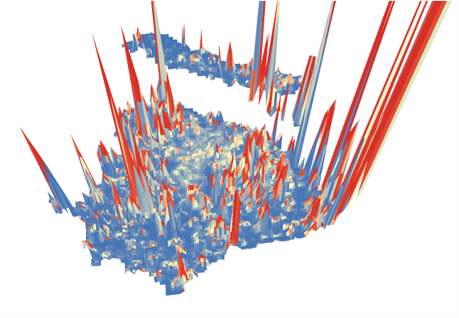
\includegraphics[width=0.68\linewidth]{3Dformat.png}
\end{generalfig}


\begin{generaltab}[htb]{人口配套性与人口分布统计}{tab:kde-pop-pop}
	\begin{tabularx}{0.9\textwidth}{p{4.2cm}ccccc}
		\toprule[1.5pt]
          & 市中心区     & 奉贤区      & 崇明区      & 浦东新区     & 金山区      \\
        \midrule
人口配套性指数   & 0.9934   & 6.0350   & 7.8034   & 1.2922   & 8.7326   \\
人口(单位:万人) & 632.9574 & 108.3463 & 70.3722  & 504.443  & 73.241   \\
\midrule[1.5pt]
& 青浦区      & 闵行区      & 嘉定区      & 松江区      & 宝山区      \\
\midrule
人口配套性指数   & 6.1106   & 2.6981   & 4.6032   & 4.2305   & 3.4653   \\
人口(单位:万人) & 108.1022 & 242.9372 & 147.1231 & 158.2398 & 190.4886 \\
		\bottomrule[1.5pt]
	\end{tabularx}
\vspace{1em}
\end{generaltab}

\subsection{现状问题总结}

(1)基于基础服务设施综合便利度

基于不同大类的基础服务设施,上海市整体的生活服务设施和休闲服务设施的空间构建还有待优化,对于服务范围覆盖率大于对市民日常生活需求影响程度的基础服务设施,应适当减少其数量或融合多个基础服务设施点的服务功能;对于服务范围覆盖率小于对市民日常生活需求影响程度的基础服务设施,应适当扩充其构建规模或扩展其服务范围与品质。从综合评价角度来看,市中心区的基础服务设施综合服务便利度较高,而近郊区与远郊的城市基础服务设施综合服务便利度较低,甚至出现0值区域。由此,上海市城市基础服务设施整体分布综合性仍需优化,不同区划的综合服务便利度仍有差异,不同类型基础服务设施服务范围覆盖程度也具有不同的优化空间。为了实现基础服务设施综合服务便利度的提升,应对未覆盖区域或综合服务便利度较低的区域进行基础服务设施补充构建,完善15分钟社区生活圈基础服务设施服务范围供给保障。

(2)基于基础服务设施人口配套性

基于不同大类的基础服务设施,结合集聚程度、服务范围覆盖率以及其对市民日常生活需求的影响程度综合分析,可得上海市整体的金融服务设施和购物服务设施的空间构建还有待优化,购物服务设施对市民日常生活有一定的需求,但其集聚程度和数量分布却较低;而金融服务设施对市民日常生活影响程度最低,但其集聚程度却高于购物服务设施。从综合评价角度来看,市中心区15分钟社区生活圈基础服务设施多样性与人口分布较为一致;而市区外围区域(主要包含宝山区、嘉定区、闵行区、松江区和浦东新区)则产生基础服务设施构建过多现象;而其他区域(主要包含青浦区、金山区和奉贤区)由于人口分布不均,其基础服务设施空间布局仍有待进一步优化。结合上海空间圈层分析可得,对于科技园区一类的特殊综合区内基础服务设施人口配套性也有明显不足。为了进一步使15分钟社区生活圈基础服务设施与人口分布贴合,再推进城市规划发展时,应结合人口分布变化,构建与之配套的基础服务设施体系。

\section{优化研究}

随着城市规划的精细化以及不断转型,注重基础服务设施均衡化配置和需求导向性配置也在逐步推进实施。15分钟社区生活圈基础服务设施是城市公共服务设施的重要组成部分,是衡量社区生活圈构建水平的重要依据,提升社区生活圈内基础服务设施服务范围覆盖率是实现公共服务均衡化的必要条件。随着市民对15分钟社区生活圈内基础服务设施的需求多元化以及居住环境宜居性要求的提升,不仅需要满足基础服务设施的服务范围在空间上的均衡分布,更需要关注因基础服务设施的供需匹配差异而造成的资源承载过量或是资源紧缺的现状;不仅需要关注基础服务设施数量的构建,更要提升基础服务设施的品质构建。本文通过寻找各类基础服务设施数量与品质和居民日常生活需求的配套发展模式,针对所归纳总结的上海市15分钟社区生活圈现有不足,从供给优化和需求匹配视角提出以下优化策略。

\subsection{基于供给优化视角策略研究}

在分类基础服务设施现有不足中,生活服务设施和购物服务设施的不足较为明显。而随着电商时代与共享基础服务设施的普及,传统购物服务设施和生活服务设施都受到了冲击,人们的生活方式和消费方式发生了变化。由此,可通过发展社区商业模式促进新型生活服务设施和购物服务设施的发展。但现有社区商业模式发展远远无法满足社区居民的日常生活对便民服务和购物服务的需求,生活服务业和购物点多为一些小卖部或是移动摊位,品种单一,品质也往往无法达到市民日常生活所需要的标准。未来,应通过构建社区商业循环提升社区生活圈内购物服务设施和生活服务设施的供给规模\textsuperscript{\cite{dong2017}}。在电子商务平台的背景下,促进线上、线下服务对接,构建线上、线下一体化的商业运营模式,打造覆盖全社区的综合服务型社区,推动智慧社区商业的发展\textsuperscript{\cite{zhu2018a}}。目前,对于社区商业模式较为主流的是社区团购商业模式,而较为主流的社区团购模式为各大电商平台配备社区团长的社区团购模式,如苏宁易购招募小区团长,主要流程如图\ref{fig:tuangou}。通过对于社区团长的培训,形成由平台仓库、团长站点和居民家三点构成的社区团购体系。在一个电商普及的时代,通过在15分钟社区生活圈内普及社区团购模式这样的社区商业模式,融合线上线下购物方式,可使实体购物服务设施的配置得到进一步优化。面对我国庞大的零售市场和高速发展的互联网技术,都为社区商业模式提供了良好的基础。社区商业模式不仅可以提升高饱和区域的实体购物服务设施的使用频率,更可以优化上海15分钟社区生活圈内购物服务设施的服务范围。随着上海等其他城市中新城区域发展的逐渐提升,社区商业模式所具有的线上下单,仓库发货以及任意距离配送特点大大减少了新城区发展后带来的资源不充足的忧虑。在未来优化发展中,构建具有高性价比物资、高效配送物流等高水平的社区商业模式,在保留适量实体购物服务设施的情况下,提升购物服务设施的品质数量和使用效率。

\begin{generalfig}[htb]{社区团购模式流程示例}{fig:tuangou}
	\vspace{1em}
	\includegraphics[width=0.9\linewidth]{tuangou.png}
	\setlength{\belowcaptionskip}{1em}   %调整图片标题与下文距离
\end{generalfig}

对于不同区划不同类别的基础服务设施优化,对未覆盖区域或综合服务便利度较低的区域进行基础服务设施补充构建,完善15分钟社区生活圈内基础服务设施服务范围的供给保障。重点关注城市边缘、城乡结合区域的基础服务设施构建,完善基础服务设施服务范围的全覆盖。在保证市中心区15分钟社区生活圈基础服务设施合理经济的服务范围的情况下,适当减少市中心区域的基础服务设施数量。在保留优质基础服务设施的现状基础上,对个别类型重复、客流量少或其他不合理基础服务设施进行撤销合并,提升城市边缘与城乡结合部的基础服务设施数量和品质。\\
%\indent 对于步行不可达区域则还可通过重构步行道路网络的方式,适当打破现有社区边界,在未来15分钟社区生活圈规划发展中,开放型的社区生活圈将成为趋势,通过社区内或社区间步行道路网络的扩充,使社区与社区之间联通,在高饱和建设区域或步行可达困难区域以联合社区共享基础服务设施的方式达到15分钟步行范围内基础服务设施的供给保障。\\
\indent 对于医疗服务设施,其服务范围覆盖率虽然达到76.07\%,但在老龄化问题日益突出的上海,医疗服务设施尤其是15分钟社区生活圈内的医疗服务设施和养老服务设施服务规模仍有待提升。在医疗服务设施分布不均衡的情况下,关注市中心区的医疗服务设施的数量和品质。通过设施职能转换、合并重构等方式改善密度较高区域的社区医疗机构。在保证服务范围覆盖率的基础上,对不符合标准的社区卫生站、诊所进行重构。对于其他区域,尤其是青浦区、奉贤区、金山区中的城市边缘区域,重点扩充医疗服务设施,加大社区医疗服务设施的构建规模。同时,关注养老设施的构建,可通过医疗服务设施结合养老服务设施的搭配模式,与医疗服务设施共同配置。在市中心区高密度、高饱和的建成环境下,提升基础服务设施品质改善居住环境,通过功能调换或是城市更新设计使得市中心区15分钟社区生活圈基础服务设施供给规模更为均衡。

\subsection{基于需求匹配视角策略研究}

市中心区从整体来看与人口配套性相较于其他区划较为一致,但也尚未达到完全匹配的情况,而市中心的高饱和用地已使得用地扩张的可能性较小,未来可能通过功能融合区域构建的方式提升15分钟社区生活圈的需求匹配。未来基础服务设施所在空间可引入“空间分时复用”模式,即分类不同年龄段的日常生活习惯(包括生活方式、出行时间段和使用不同类别基础服务设施的时间差),通过对同一基础服务设施点的不同时间段设置不同功能,如在工作日的工作时间可以设置针对于老年的基础服务设施;而在工作日的夜晚可以构建针对年轻人或儿童的基础服务设施功能。通过将面向不同年龄段的基础服务功能在空间位置上融合,以共享使用和共同布局的方式,提高设施使用效率,提升15分钟社区生活圈内基础服务设施品质,具体案例见图\ref{fig:multifunction}。对于某一待优化的空间区域,其原有基础服务设施可能仅为单一的主要适合老年人的休闲服务设施,在优化过程中,可以添加适合儿童的休闲服务设施,使该区域可在下午时段(如13:00至15:00)为携带幼儿或有照看幼儿需求的老人或相关人群提供相应便利;在该区域还可添加一些简单的餐饮服务设施,如流动餐车、或者是简单的餐饮服务窗口,不仅可在晚间时段(如19:00至22:00)为成年人如下班族提供一些简单的餐饮服务,也可为其他时段需要相应需求的人群提供相应的服务。

\begin{generalfig}[htb]{空间分时复用模式举例}{fig:multifunction}
	\vspace{1em}
	\includegraphics[width=0.92\linewidth]{multifunction.png}
	%\setlength{\belowcaptionskip}{1em}   %调整图片标题与下文距离
\end{generalfig}

对于市中心区,还可通过打破原本社区边界,融合相邻社区,补充构建社区步行道路网络提升15分钟社区生活圈的需求匹配。鼓励社区生活圈用地规模塑造成 2~4 公顷的居住团体规模,打造开放的社区空间,提升社区之间的活力,满足居民日益多元的基础服务设施需求和对居住环境宜居性的追求\textsuperscript{\cite{liu2019}}。对于其他区划的基础服务设施人口配套性,不仅需要注意基础服务设施的品质,更应保证随着五大新城和上海道路网络的扩张所改变的人口分布而改变的市民需求规模。未来可通过优化分级基础服务设施体系提升15分钟社区生活圈内基础服务设施人口配套性。\\
\indent 以医疗设施为例,现有的社区医疗设施服务水平往往不能达到市民日常生活所需的水平,即改善社区医疗服务水平,进而提高社区医疗设施使用效率,解决医疗卫生设施供需矛盾。未来,通过将社区医院作为医疗服务设施体系构建的重点,通过医疗资源的整合,构建分级配套的优质医疗服务设施体系,建立以医院为核心、药店为基础、社区卫生设施点为保障的15分钟社区生活圈优质医疗服务设施体系。提高社区医疗服务人员待遇,引导高素质人才输送社区医院,优化社区医疗人才素质结构,强调“社区首诊制”(见图\ref{fig:multilevelmedicine}),即使患者(如对自己身体状况较为了解的成年群体或是定期配药的老年群体)首先在生活圈内基层医疗服务设施就诊,并根据就诊情况判断是否需要转诊,也可通过医疗资源共享以及患者情况的数字化建设与实时沟通,使15分钟社区生活圈可以提供更完整高效的医疗服务,不仅提升15分钟社区生活圈中医疗服务设施使用效率更可为患者提供省时省力的便利。对于医疗服务设施,还可将其与养老结合制度,利用互联网技术联通高层级医院技术资源优势,开展特色服务,强化保健、康复、护理、健康教育等功能,实现医疗基础服务设施供需匹配的提升\textsuperscript{\cite{ji2018}}。

\begin{generalfig}[htb]{“社区首诊制”模式示意图}{fig:multilevelmedicine}
	\vspace{1em}
	\includegraphics[width=0.92\linewidth]{multilevelmedicine.png}
	%\setlength{\belowcaptionskip}{1em}   %调整图片标题与下文距离
\end{generalfig}

随着15分钟社区生活圈这一理念在我国城市规划体系中的不断深入影响,15分钟社区生活圈的构建框架也在不断摸索中优化。不仅需要关注现存问题并制定相对应的优化策略,更需要各领域的配合。不仅需要完善基础服务设施的空间布局,更需要制定良好的管理方法来保障15分钟社区生活圈规划构建。对于细化尺度下的15分钟社区生活圈构建将是未来研究的重点,在现有研究中也已经有针对不同区划的不同实施方案开展初步探索\textsuperscript{\cite{xu2019}}。在实施方案的同时,还应逐步加深跨学科知识的融合,加深居民这一社区居住主体的参与,带动居民积极参与所住环境的建设,打造活力社区,将在未来的15分钟社区生活圈规划中越来越重要。

\section{本章小结}

本章首先选取典型街道:田林街道和曲阳路街道,通过对比统计数据处理结果和运用模型所得结果,得到平均数据一致性为98.1\%,即本模型具有较高可信度,适合文本研究内容,也指出了本文模型验证方法的不足以及未来改进方向。

在此基础上,运用所构建模型评价上海市15分钟社区生活圈现状并基于15分钟社区生活圈基础服务设施综合服务便利度和15分钟社区生活圈基础服务设施人口配套性视角归纳总结出现有不足:(1)从分类基础服务设施来看,上海市整体生活服务设施和购物服务设施的空间布局还有待优化。(2)从综合评价角度,市中心区的基础服务设施综合服务便利度较高,而近郊区与远郊的基础服务设施综合服务便利度较低;市中心区15分钟社区生活圈基础服务设施多样性与人口分布较为一致;而市区外围区域(主要包含宝山区、嘉定区、闵行区、松江区和浦东新区)则产生基础服务设施构建过多现象;而其他区域(主要包含青浦区、金山区和奉贤区)由于人口分布不均,其基础服务设施空间布局仍有待进一步优化。此外,上海科技园区一类的特殊综合区内基础服务设施人口配套性也有明显不足。

基于以上不足,从供给优化视角提出以下优化策略:(1)对于生活服务设施和购物服务设施,可通过发展社区商业模式促进新型生活服务设施和购物服务设施的发展。(2)对于不同区划不同类别的基础服务设施优化,重点关注城市边缘、城乡结合区域的基础服务设施构建,完善基础服务设施服务范围的全覆盖,适当减少市中心区域的基础服务设施数量。(3)对于医疗服务设施,通过设施职能转换、合并重构等方式改善社区医疗机构。从需求匹配视角提出如下优化策略:(1)对于市中心区,通过功能融合区域构建或打破原本社区边界,融合相邻社区,补充构建社区步行道路网络的方式提升15分钟社区生活圈的需求匹配并以“空间分时复用”模式为例阐述了具体可实施方案。(2)对于其他区划,优化分级基础服务设施体系提升15分钟社区生活圈内基础服务设施人口配套性并以医疗服务设施“社区首诊制”为例阐述分级优化基础服务设施可实施方案。
	
%%%%%%%%%%%%%%%%%%%%%%%%%%%%% 第五章  %%%%%%%%%%%%%%%%%%%%%%%%%%%%%%%%

\chapter{结论与展望}

\section{结论}

本文基于城市多源空间数据集,融合网络分析法、熵值法、线性加权法、标准差椭圆、核密度分析法、比值法等地理空间分析模型和统计模型,构建15分钟社区生活圈评价模型和评价指标体系,并根据所得结果归纳总结现存不足后提出相应的优化策略。所得现存不足主要表现为以下几个方面:(1)从分类基础服务设施来看,上海市整体生活服务设施和休闲服务设施的空间构建还有待优化。(2)从综合评价角度,市中心区的基础服务设施综合服务便利度较高,而近郊区与远郊的城市基础服务设施综合服务便利度较低;市中心区15分钟社区生活圈基础服务设施多样性与人口分布较为一致;而市区外围区域(主要包含宝山区、嘉定区、闵行区、松江区和浦东新区)则产生基础服务设施构建过多现象;而其他区域(主要包含青浦区、金山区和奉贤区)由于人口分布不均,其基础服务设施空间布局仍有待进一步优化。此外,上海科技园区一类的特殊综合区内基础服务设施人口配套性也有明显不足。基于以上不足,从供给优化视角提出以下优化策略:(1)对于生活服务设施和购物服务设施,可通过发展社区商业模式促进新型生活服务设施和购物服务设施的发展。(2)对于不同区划不同类别的基础服务设施优化,重点关注城市边缘、城乡结合区域的基础服务设施构建,完善基础服务设施服务范围的全覆盖,适当减少市中心区域的基础服务设施数量。(3)对于医疗服务设施,通过设施职能转换、合并重构等方式改善社区医疗机构。从需求匹配视角提出如下优化策略:(1)对于市中心区,通过功能融合区域构建或打破原本社区边界,融合相邻社区,补充构建社区步行道路网络的方式提升15分钟社区生活圈的需求匹配。(2)对于其他区划,优化分级基础服务设施体系提升15分钟社区生活圈内基础服务设施人口配套性。本文基于“以人为本”理念构建15分钟社区生活圈评价模型和评价指标体系,并以上海为例展开研究,基于供需匹配视角归纳现存不足并提出相应优化策略,试图探索可复制的15分钟社区生活圈规划模型,使之可推广至长三角城市群,为进一步开展15分钟社区生活圈研究提供参考意见,推进可持续发展理念下的城市建设。

\section{研究创新点}

(1)引入多源城市空间数据集

本文通过引入多源城市空间数据集,使15分钟社区生活圈研究更加全面。本文通过引入多类基础服务设施数据使15分钟社区生活圈评价更综合;本文引入城市路网数据,基于城市路网即开展基于网络的空间分析,更符合日常生活的实际情况;本文引入人口分布数据,更能体现15分钟社区生活圈规划“以人为本”的核心。与现有研究相比,引入多源城市空间数据集,丰富15分钟社区生活圈研究数据源,不仅使研究考量更全面,研究结果更贴近现实生活,所提出的优化结果也更具可信度。

(2)构建基于市民日常生活需求的评价模型和评价指标体系

本文将市民需求和人口空间分布特征纳入15分钟社区生活圈的考量范畴。通过调查问卷和熵值法将市民对不同类别基础服务设施的需求程度转化为不同类别基础服务设施的权重,并加入15分钟社区生活圈评价模型的构建。通过权重和不同类别基础服务设施服务范围的融合得到15分钟社区生活圈基础服务设施综合服务便利度;结合权重和不同类别基础服务设施空间分布特征得到15分钟社区生活圈基础服务设施混合多样性体现特定区域内15分钟社区生活圈基础服务设施的种类丰富程度和市民需求是否符合。通过计算人口空间分布和基础服务设施混合多样性的比值,得出15分钟社区生活圈内基础服务设施与人口分布的配套性,体现特定区域内15分钟社区生活圈基础服务设施配置是否合理。与现有15分钟社区生活圈评价模型相比,本文构建模型更加关注15分钟社区生活圈内基础服务设施的需求导向配置,更符合自下而上,市民参与的“以人为本”的15分钟社区生活圈规划理念。

\section{不足与展望}

本文以上海为例,初步探索15分钟社区生活圈基础服务设施与市民关注、感知与需求之间的相互关系,并构建相应模型与评价指标体系评价现状后提出对应的优化策略,但仍有以下方面有待进一步优化。

(1)从数据的角度来看,本文使用OSM作为城市步行网络数据源。OSM数据虽然已经是一个相对成熟的志愿者地理信息服务,但其数据仍有一定程度的主观性,拓扑结构和对城市覆盖度仍有待进一步筛选与补充;本文使用LandScan作为人口分布数据源,虽然考虑了其在空间位置分布的准确度,但对其空间分辨率的优化仍有待进一步挖掘,在之后的研究中,可通过引入其他数据(如Worldpop或夜间灯光数据)辅助构建更高分辨率的人口数据源,使之在15分钟社区生活圈的研究中应用推广。本文通过关注市、区级的行政区划来开展研究,将不同社区所构成的区看作一个整体,但不同的社区对基础服务设施也有不同的要求。此外,上海经常有新旧社区,对于新社区,只需通过一些社区微更新项目优化15分钟社区生活圈的建设;对于一些老旧社区,需要通过综合评价形成改造方案。在现有研究中,也已经对此有了初步的案例研究,如浦东陆家嘴社区的案例\textsuperscript{\cite{zhao2018}}。在之后的研究中,通过对于社区边界数据的补充以及对模型完成相应优化后,可使研究进一步细化,提出可供社区实施的15分钟社区生活圈优化策略。

(2)本文已初步关注将“以人为本”纳入15分钟社区生活圈规划、评价与优化中,但对于“人”仅初步关注了市民整体对所居住环境中设施的感知与需求,而尚未细化关注不同人群的不同关注与影响。不同年龄层次的人群,甚至不同特征的人群(如上班族、学生等),对15分钟社区生活圈的基础服务设施配置有不同的要求。例如,在工作日,上班族对夜间开放的基本服务设施的需求较高,尤其是餐饮与生活服务设施,如24小时便利店;而老年人则不同,他们需要的是基于家庭服务和休闲娱乐的基础服务设施,如超市、菜市场、活动室等。在未来的研究中,应以年龄为主要因素,划分不同人群对不同基础服务设施的需求,并在此基础上对于公共服务设施的配置应进一步关注老年人、儿童等弱势群体的需求。对于老年人占主导地位的社区(例如,60岁以上老年人口达到总人口的25\%以上的社区或老年人超过80岁人口占10\%以上),15分钟社区生活圈基本服务设施的使用可以根据老年人的生活方式在不同时段进行调整\textsuperscript{\cite{huang2019a}}。对于儿童比例较高的社区(这可以由出生率决定),应该考虑儿童可参与的基础服务设施的配套情况(包含安全性和未来发展)\textsuperscript{\cite{peng2020}}。在之后的研究中,通过对人口分类数据的补充完善,也将进一步开展对不同年龄段友好型社区的研究。\\
\indent (3)本文所关注的基础服务设施类别主要包含餐饮服务设施、购物服务设施、生活服务设施、医疗服务设施、休闲服务设施、金融服务设施,初步探索15分钟社区生活圈内基础服务设施的综合评价。随着城市规划转型和人民对更高生活质量的追求,基于马斯洛需求层次理论,不仅需要的是生理层面的需求,安全层面的需求(如文化、健康保障)也应被纳入15分钟社区生活圈规划决策之中,提升对应的基础服务设施品质。2020,面对全球新冠疫情也再一次让我们意识到健康社区的重要性。许多研究已经证明,健康智慧社区的建设会影响居民的运动态度,进而影响公民的健康\textsuperscript{\cite{lovasi2011}}。在现有研究中,国内外相关学者也已经开始逐步关注健康社区这一理念,并展开相关的规划研究,制定相关评价标准。在国际上,已经提出WELL社区标准作为第一个试运行的全球标准发布,提出以健康、包容、公平、全面、活力为基础的规划标准\textsuperscript{\cite{li2019a}},与15分钟社区生活圈相关的标准归纳如图\ref{fig:wellcommunity}。在我国,对于疫情后的社区生活圈研究框架也已经有了初步的探讨\textsuperscript{\cite{shen2020,chai2020}}。

\begin{generalfig}[htb]{与15分钟社区生活圈相关的WELL COMMUNITY标准}{fig:wellcommunity}
	\includegraphics[width=0.92\linewidth]{wellcommunity.png}
\end{generalfig}

在之后的研究中,本文也将通过完善模型,关注医疗服务设施的均衡布局,深入实施“健康上海”,提升突发公共卫生事件应对能力,加强市民健康保障。本文对于基础服务设施类别的关注也仅是初步关注了以功能为划分的分类,尚未关注更细化分级的基础服务设施。同一特征群体对不同分级的基础服务设施的需求不同。以医疗服务设施大类为例,不同级别的医疗服务设施所对应的使用人群不同。如老年群体的日常生活需求可能更多的是社区医院的药物获取,即对基层级别医疗服务设施的需求较多。而对于规模大、高水平医疗服务设施(如三甲医院)的需求更多来自与外来人口的疑难杂症的就诊。在之后的研究中,也将细化不同特征人群对不同分级基础服务设施的需求,使研究结果更贴近15分钟社区生活圈内的日常生活情况和市民日常生活习惯。



% 主体部分结束啦

%%%%%%%%%%%%%%%%%%%%%%%%%%%%%%%%%%%%%%%%%%%%%%%%%%%%%%%%%%%%%%%%%%%%%%%%%%

\backmatter  % 结束章节自动编号

%%%%%%%%%%%%%%%%%%%%%%%% 生成参考文献  %%%%%%%%%%%%%%%%%%%%%%%%%%%%%%%%%%%%%

\bibliographystyle{thuthesis-numeric}
%\bibliographystyle{shnuthesis-numeric}
\bibliography{mybib}

%%%%%%%%%%%%%%%%%%%%%%%% 附录  %%%%%%%%%%%%%%%%%%%%%%%%%%%%%%%%%%%%%%%

%无附录
%添加附录, 如不需要可以注释掉
%\appendix

%%%%%%%%%%%%%%%%%%%%%% 攻读硕士学位期间的研究成果  %%%%%%%%%%%%%%%%%%%%%%%%%%%

\begin{researchpage}
[1] 郭华东 . 地球大数据支撑可持续发展目标报告 [R]. 北京: 中国科学院, 2021.(将于2021年9月发布)
[参与编写案例:中国城市公共空间评估]

[2]Wu~H, Wang~L, Zhang Z, et al. Analysis and optimization of 15-minute community life circle based on supply and demand matching: A case study of Shanghai. PlosONE. (submitted)

\end{researchpage}


%%%%%%%%%%%%%%%%%%%%%%%%%%% Thanks page %%%%%%%%%%%%%%%%%%%%%%%%%%%%%%%%%%%%

\begin{thankpage}
\chaptermark{致谢}
\setlength{\baselineskip}{24pt}
	
三月的最后一天,论文进入尾声,这也就意味着即将毕业。回忆过往,不知不觉在学校的七年即将画上句号。从本科伊始的懵懵懂懂,也随着不断地积累与沉淀到如今逐渐沉稳。七年,和身边的同学经历了相遇到离别,在学习与研究中也曾有过迷茫到坚定,感慨良多,收获良多。在以后的生活中,我们还是会遇到或艰难,或幸运,但这七年的时光所获得的都将化为一份财富伴随我们永远。

经师易得,人师难求。桃李不言,下自成蹊。七年之间,致敬并感恩遇到的每一位老师。最想感谢的是我的导师王亮绪老师,对每一份数据的严谨、细致,对每一稿论文的高标准,以认真踏实的学术态度和务实专注的人生态度影响着我们不断追逐和进步,不断体验和学习新知。在每一次的师门组会中教学与培养我们的科研素养,在每一次的论文修改讨论中为我们传道与解惑。在生活中,老师平易近人,为人着想,感谢老师对我学习和生活上的关心,是对下一阶段迷茫时给予自信和坚定,是在挫折时给与鼓励与引导,言传身教影响着我处世与生活,以身作则教会我淡泊真心待人。毕业之际,感谢您对我就业规划、个人发展的指导和帮助,感谢您从论文撰写、修改到定稿对我的指导。此外,特别感谢张中浩老师在科研竞赛中对我们的帮助与指导。同时,感谢每一位授课老师,是你们使我们对专业有了进一步的认知。最后,感谢七年来遇见的每一位老师,师恩难忘!

感谢七年来相知相遇的每一位同学,特别是杨文雪、王笑寒、范择东等相伴七年的同学,从奉贤到徐汇,从学海路到桂林路,一起熬夜,一起考研,一起写论文,一起分享着生活中的点滴,一起走过这段岁月。感谢你们愿意在深夜倾听那些糟心事,感谢你们在低谷时给予的陪伴与安慰,感谢你们对于日常生活中的帮助与理解。感谢我的同门师姐、师弟。在科研中一起讨论、解决问题、交流心得,建立真挚的同门情谊。祝七年来所有遇见的同学一切顺利,友情长存。感恩相遇!

最后,感谢我的父母和我所有的家人,是你们一路陪伴我走到现在,一直包容我、支持我,使我能勇敢的完成每一个想法和决定,成为我最坚强的后盾。

再次衷心致谢所有在这七年来出现过的人和事,你们的存在使我的人生更加充实丰富,祝平安喜乐,万事顺意。

满目山河,明天还要赶很远的路。愿心怀感恩,身怀所学,能成为各自想成为的人。不忘初心,乘风破浪,体验这草木一生。

\rightline{2021年3月}
	
\end{thankpage}

%%%%%%%%%%%%%%%%%%%%%%%%%%%%%  OKK  %%%%%%%%%%%%%%%%%%%%%%%%%%%%%%%%%

\end{document}



